% =====================================================================================
%  Case-study workbook: load flow, operating limits and renewable integration with PyPSA
%  Same layout as the "Fiche de methode: le systeme per unit".   Compile: pdflatex (x2)
% =====================================================================================
\documentclass[11pt,a4paper]{article}
\usepackage[T1]{fontenc}
\usepackage[utf8]{inputenc}
\usepackage{lmodern}
\usepackage{tgtermes}
\usepackage[english]{babel}
\usepackage[a4paper,top=2.6cm,bottom=2.6cm,left=2.5cm,right=2.5cm,headheight=14pt]{geometry}
\usepackage{amsmath,amssymb}
\usepackage{graphicx}
\usepackage{booktabs,array,tabularx,multirow}
\usepackage{caption}
\usepackage{xcolor}
\usepackage{listings}
\usepackage{enumitem}
\usepackage{titlesec}
\usepackage{fancyhdr}
\usepackage[most]{tcolorbox}
\usepackage{tikz}
\usetikzlibrary{arrows.meta,calc,positioning}
\usepackage{microtype}
\usepackage[hidelinks]{hyperref}

\graphicspath{{figures/}{../results/figures/}}
\setlength{\parindent}{0pt}
\setlength{\parskip}{5pt}
\setlist{nosep,leftmargin=1.5em}
\captionsetup{font=small,labelsep=colon}
\captionsetup[table]{position=top}

% ---------------------------------------------------------------- header and sections
\pagestyle{fancy}
\fancyhf{}
\fancyhead[L]{\small Case-study workbook: load flow and planning with PyPSA}
\fancyhead[R]{\small KOUAME Koffi Fidèle, IMP-EGH}
\fancyfoot[C]{\small\thepage}
\renewcommand{\headrulewidth}{0.4pt}
\titleformat{\section}{\large\bfseries}{\thesection.}{1em}{}
\titleformat{\subsection}{\normalsize\bfseries}{}{0em}{}
\titlespacing*{\section}{0pt}{18pt}{8pt}
\titlespacing*{\subsection}{0pt}{10pt}{4pt}

% ---------------------------------------------------------------- boxes (grey title bar)
\newtcolorbox{gbox}[1]{enhanced, colback=white, colframe=gray!45, colbacktitle=gray!22,
  coltitle=black, fonttitle=\bfseries, title={#1}, sharp corners, boxrule=0.5pt,
  left=6pt, right=6pt, top=4pt, bottom=4pt, before skip=8pt, after skip=8pt}
\newtcolorbox{sayit}{enhanced, colback=gray!7, colframe=gray!7, sharp corners,
  left=8pt, right=8pt, top=5pt, bottom=5pt, before skip=8pt, after skip=8pt,
  title={What I say in front of a jury}, colbacktitle=gray!7, coltitle=black, fonttitle=\bfseries\itshape}

% ---------------------------------------------------------------- code listings
\lstdefinestyle{py}{language=Python, basicstyle=\ttfamily\scriptsize, keywordstyle=\bfseries,
  commentstyle=\itshape\color{gray!70!black}, stringstyle=\color{black!75},
  backgroundcolor=\color{gray!6}, frame=single, rulecolor=\color{gray!40}, framesep=4pt,
  numbers=left, numberstyle=\tiny\color{gray}, numbersep=6pt, xleftmargin=14pt,
  breaklines=true, columns=fullflexible, keepspaces=true, showstringspaces=false,
  upquote=true, literate={->}{{$\rightarrow$}}2}
\lstdefinestyle{out}{basicstyle=\ttfamily\scriptsize, backgroundcolor=\color{white},
  frame=leftline, rulecolor=\color{gray!60}, framerule=1.5pt, xleftmargin=6pt,
  breaklines=true, columns=fullflexible, keepspaces=true, showstringspaces=false}
\newcommand{\code}[2]{\lstinputlisting[style=py,caption={#2}]{../solutions/#1}}
\newcommand{\progout}[2]{\lstinputlisting[style=out,caption={#2}]{../solutions/output/#1}}
\renewcommand{\lstlistingname}{Code}

% ---------------------------------------------------------------- one-line diagram styles
\tikzset{
  bus/.style={line width=2.4pt},
  ln/.style={line width=0.8pt},
  gen/.style={circle, draw, line width=0.8pt, minimum size=9mm, inner sep=0pt, font=\small},
  load/.style={-{Stealth[length=2.6mm]}, line width=0.8pt},
  lab/.style={font=\footnotesize, fill=white, inner sep=1.5pt},
  res/.style={font=\footnotesize\bfseries, inner sep=1pt},
}

\begin{document}

% ================================================================ title block (as the fiche)
\begin{center}
{\LARGE\bfseries CASE-STUDY WORKBOOK}\\[3pt]
{\Large Load flow, operating limits and renewable integration with PyPSA}\\[6pt]
{\small Power System Modeling, Simulation and Control \quad$|$\quad Sources: Exercise 5 (28 October 2022);
Travaux pratiques ``Load flow on a real network''; H.\ Saadat, \emph{Power System Analysis}; PyPSA 1.4}
\end{center}
\vspace{-4pt}\noindent\rule{\textwidth}{0.6pt}

\section{How every case is solved: the scientific approach}

Each exercise is treated in the same eight steps. The steps are the same for a three-bus
textbook network and for a full year of real weather: only the data and the questions change.

\begin{gbox}{Method: the eight steps applied to every case}
\begin{enumerate}
\item \textbf{Statement and question}: the exercise as given, with its original diagram; the engineering question it asks.
\item \textbf{Data and hypotheses}: every number used, its unit, its source, and every assumption made.
\item \textbf{Physical model}: the equations that link the unknowns to the data (load-flow equations, limits, costs).
\item \textbf{Solution method}: the algorithm (Newton-Raphson, optimal power flow, N-1 screening, bisection on a limit).
\item \textbf{Implementation in PyPSA}: the complete, commented Python code (also in \texttt{solutions/}).
\item \textbf{Results}: the printed output of that code, tables and figures.
\item \textbf{Verification}: an independent check (hand calculation, own solver, energy balance, physical plausibility).
\item \textbf{Interpretation and recommendation}: what the numbers mean for the grid, and what to do.
\end{enumerate}
\end{gbox}

\subsection{PyPSA in five objects}
\begin{table}[h]\centering\small
\caption{The PyPSA objects used in this workbook.}
\resizebox{\textwidth}{!}{\begin{tabular}{@{}lll@{}}
\toprule
Object & What it represents & Key attributes \\
\midrule
\texttt{n = pypsa.Network()} & the grid & \texttt{n.snapshots} (time steps) \\
\texttt{n.add("Bus", ...)} & a node & \texttt{v\_nom} (kV), \texttt{v\_mag\_pu\_set} (PV/slack set point) \\
\texttt{n.add("Line", ...)} & a branch ($\pi$ model) & \texttt{r}, \texttt{x} ($\Omega$), \texttt{b} (S), \texttt{s\_nom} (MVA) \\
\texttt{n.add("Generator", ...)} & an injection & \texttt{control} = Slack / PV / PQ, \texttt{p\_set}, \texttt{q\_set}, costs \\
\texttt{n.add("Load", ...)} & a consumption & \texttt{p\_set} (MW), \texttt{q\_set} (MVAr) \\
\midrule
\texttt{n.pf()} & AC load flow (Newton-Raphson) & results in \texttt{n.buses\_t.v\_mag\_pu}, \texttt{n.lines\_t.p0} \dots \\
\texttt{n.optimize()} & optimal power flow / investment & results in \texttt{n.generators\_t.p}, \texttt{p\_nom\_opt} \\
\bottomrule
\end{tabular}}
\end{table}

\begin{gbox}{Link with the per-unit method sheet: from p.u.\ to the units of PyPSA}
PyPSA stores line data in physical units. With the base of the zone of the line (same rule as in the per-unit sheet):
\[ Z_B = \frac{(\text{kV}_B)^2}{\text{MVA}_B}, \qquad r_\Omega = r_{pu}\,Z_B, \qquad x_\Omega = x_{pu}\,Z_B, \qquad b_S = \frac{b_{pu}}{Z_B}. \]
Example (Exercise 5): $S_B = 100$ MVA, $V_B = 110$ kV, $Z_B = 121\ \Omega$; $X = 0.125$ p.u.\ $\Rightarrow$ $15.125\ \Omega$; $B^0 = 0.1$ p.u.\ $\Rightarrow$ $8.26\times10^{-4}$ S.
The p.u.\ results do not depend on the choice of $V_B$.
\end{gbox}

% ================================================================ Exercise 5 - A1
\section{Exercise 5, Assignment 1: Newton's method}

\subsection{Step 1: statement and question}
\begin{gbox}{Statement}
Perform 5 iterations using Newton's method to solve $f(x) = 10x^2 - 2x^3 = 0$. The answer should
include the expression for the derivative $f'(x)$ and the values of $x$, $\Delta x$, $f(x)$ and
$f'(x)$ at each iteration. (a) Start at $x = 1$. (b) Start at $x = 4$. (c) Sketch $f(x)$ versus $x$
to see the graphical solutions.
\end{gbox}
\textbf{Question behind the exercise:} how does the algorithm used by every load-flow program behave,
and why does its starting point matter?

\subsection{Step 2: data and hypotheses}
$f(x) = 10x^2 - 2x^3 = 2x^2(5 - x)$: two roots, $x = 0$ (double) and $x = 5$ (simple). No hypothesis is needed.

\subsection{Step 3: model}
\[ f'(x) = 20x - 6x^2 = 2x(10 - 3x), \qquad \Delta x_k = -\frac{f(x_k)}{f'(x_k)}, \qquad x_{k+1} = x_k + \Delta x_k. \]
$f'$ vanishes at $x = 0$ and $x = 10/3$: there the tangent is horizontal and no step can be computed.

\subsection{Step 4: method}
Newton replaces $f$ by its tangent at $x_k$ and jumps to the zero of the tangent. Simplified update:
$x_{k+1} = x_k\,\dfrac{10 - 4x_k}{20 - 6x_k}$, which tends to $x_k/2$ near 0.

\subsection{Step 5: implementation}
\code{s01_newton_method.py}{Newton's method, Exercise 5 Assignment 1.}

\subsection{Step 6: results}
\progout{s01.txt}{Output of Code 1.}

\begin{figure}[h]\centering
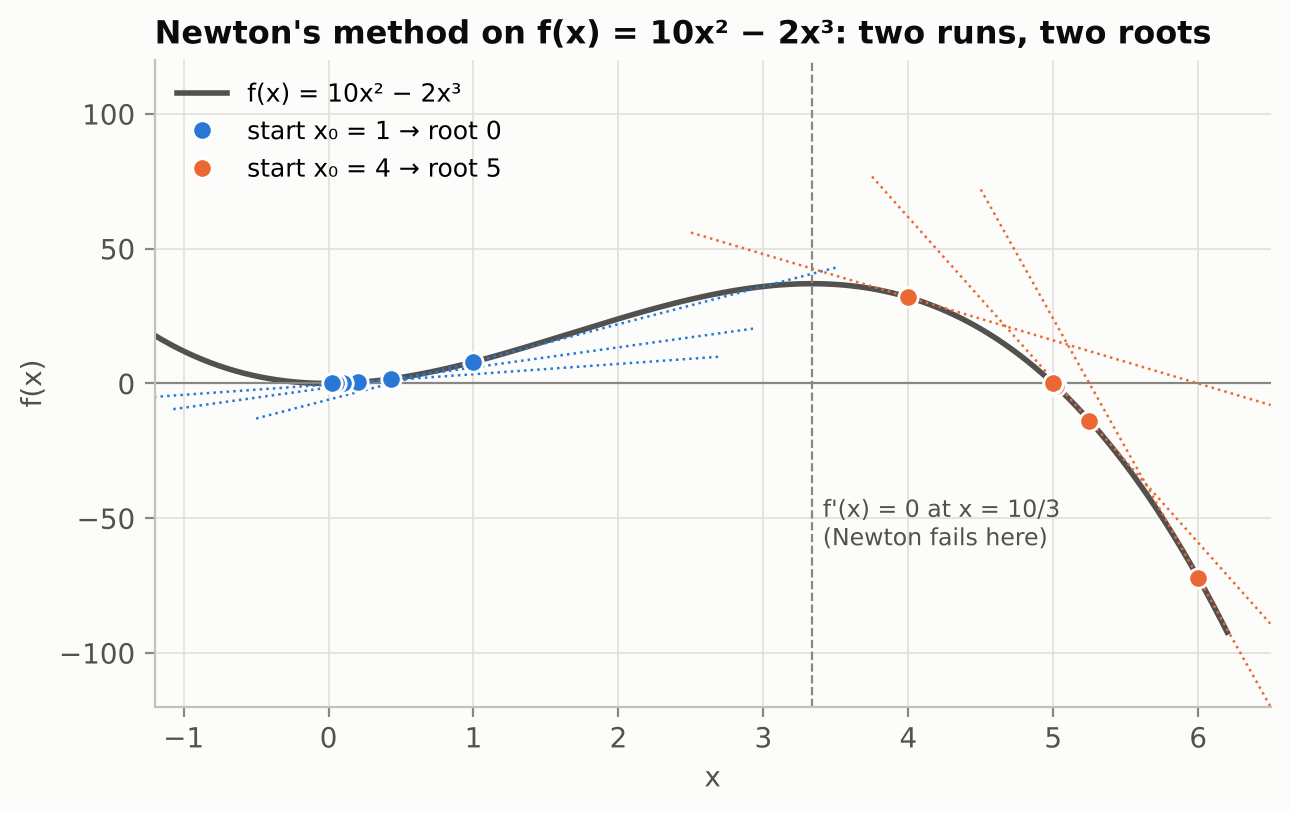
\includegraphics[width=0.72\textwidth]{cs00_newton_function.png}
\caption{Question (c): $f(x)$, the iterates of both runs and the first tangents.}
\end{figure}

\subsection{Step 7: verification}
Hand check of the first step from $x_0 = 1$: $f(1) = 8$, $f'(1) = 14$, $\Delta x = -0.5714$, $x_1 = 0.4286$ (same as the output).
From $x_0 = 4$: $f(4) = 32$, $f'(4) = -16$, $\Delta x = +2$, $x_1 = 6$. The final values are roots: $f(0.0245) \approx 0.006$, $f(5.00000001) \approx -5\times10^{-7}$.

\subsection{Step 8: interpretation}
\begin{itemize}
\item From $x_0 = 1$ the method converges to the \textbf{double root 0}, but \textbf{linearly}: $e_{k+1}/e_k \to 0.5$, after 5 steps $x = 0.0245$.
\item From $x_0 = 4$ it overshoots to 6 (negative slope), then converges \textbf{quadratically} to 5: $e_{k+1}/e_k^2 \to 0.4$, 8 exact digits after 5 steps.
\item At $x_0 = 10/3$, $f' = 0$: the method fails. The root found depends on the starting point.
\end{itemize}
\begin{sayit}
``A load flow is a vector version of this method: the Jacobian replaces $f'(x)$. A flat start is a good first guess because grids run near 1 p.u.; quadratic convergence explains why a load flow needs only 3 to 5 iterations; and a singular Jacobian, like $f' = 0$ here, marks the voltage-collapse point.''
\end{sayit}

% ================================================================ Exercise 5 - A2
\section{Exercise 5, Assignment 2: Newton-Raphson load flow of a three-bus grid}

\subsection{Step 1: statement and question}
\begin{gbox}{Statement}
The one-line diagram of a three-phase system with three nodes is shown in Figure~\ref{fig:ex5}. Bus 1
is the balance (slack) bus, node 2 a generator bus and node 3 a load bus.
(1) Determine the node admittance matrix. (2) Derive the load-flow problem and solve it with the
Newton-Raphson method. (3) Determine the power flows and transmission losses.
\end{gbox}
\begin{figure}[h]\centering
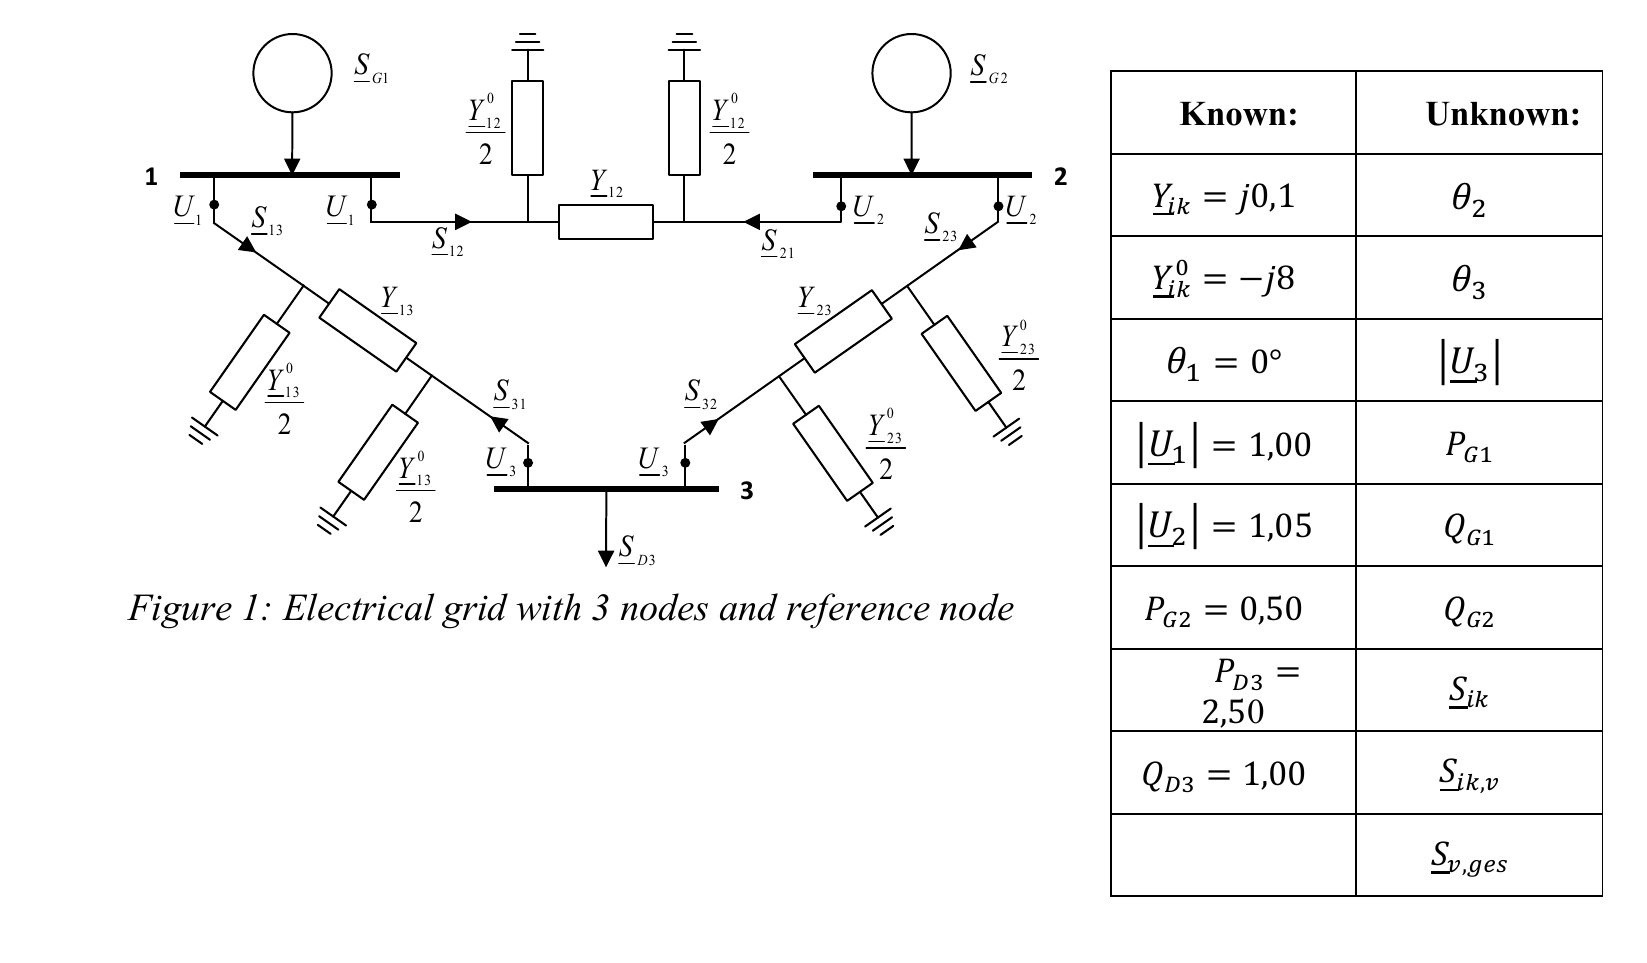
\includegraphics[width=0.95\textwidth]{ex5_original_figure1.png}
\caption{Original figure and data table of Exercise 5 (Figure 1: electrical grid with 3 nodes and reference node).}\label{fig:ex5}
\end{figure}

\subsection{Step 2: data and hypotheses}
\begin{table}[h]\centering\small
\caption{Exercise 5: data used (p.u., $S_B = 100$ MVA).}
\begin{tabular}{@{}llll@{}}
\toprule
Bus & Type & Known & Unknown \\
\midrule
1 & slack & $|U_1| = 1.00$, $\theta_1 = 0^\circ$ & $P_{G1}$, $Q_{G1}$ \\
2 & PV & $|U_2| = 1.05$, $P_{G2} = 0.50$ & $\theta_2$, $Q_{G2}$ \\
3 & PQ & $P_{D3} = 2.50$, $Q_{D3} = 1.00$ & $\theta_3$, $|U_3|$ \\
\midrule
Lines 1-2, 1-3, 2-3 & $\pi$ model & series $\underline Y_{ik} = -j8$; shunt $\underline Y^0_{ik} = j0.1$ ($j0.05$ per end) & flows, losses \\
\bottomrule
\end{tabular}
\end{table}

\begin{gbox}{Hypothesis on the line data (to state on the exam paper)}
The table gives $\underline Y_{ik} = j0.1$ and $\underline Y^0_{ik} = -j8$. Taken literally, the series element would be a
capacitor and the shunt an 8 p.u.\ reactor; the problem then has \textbf{no solution} (a series admittance of 0.1 p.u.\
cannot carry 2.5 p.u.; Newton diverges). The physically consistent reading swaps the two values:
series admittance $-j8$ (an inductive line, $X = 0.125$ p.u.) and line charging $+j0.1$. Reading both values as
impedances ($Z = j0.1$, $Z^0 = -j8$) gives $|U_3| = 0.971$ p.u.: the conclusions are the same.
\end{gbox}

\subsection{Step 3: model}
\textbf{Admittance matrix.} Each line adds $\underline y_{ik} + \underline Y^0_{ik}/2$ to $Y_{ii}$ and $Y_{kk}$, and $-\underline y_{ik}$ to $Y_{ik}$. Each bus has two lines:
\[ Y_{ii} = 2(-j8) + 2(j0.05) = -j15.9, \qquad Y_{ik} = +j8, \qquad
\mathbf Y = \begin{bmatrix} -j15.9 & j8 & j8 \\ j8 & -j15.9 & j8 \\ j8 & j8 & -j15.9 \end{bmatrix}. \]
\textbf{Load-flow equations} (lossless lines, $G = 0$, $B_{ik} = 8$, $B_{ii} = -15.9$):
\begin{align*}
P_2 &= 8|U_2||U_1|\sin\theta_{21} + 8|U_2||U_3|\sin\theta_{23} = +0.50\\
P_3 &= 8|U_3||U_1|\sin\theta_{31} + 8|U_3||U_2|\sin\theta_{32} = -2.50\\
Q_3 &= 15.9|U_3|^2 - 8|U_3||U_1|\cos\theta_{31} - 8|U_3||U_2|\cos\theta_{32} = -1.00
\end{align*}
Three equations, three unknowns $x = [\theta_2, \theta_3, |U_3|]^T$. There is no $Q_2$ equation: bus 2 is a PV bus.

\subsection{Step 4: method (first iteration by hand)}
Flat start: $\theta_2 = \theta_3 = 0$, $|U_3| = 1$. Computed injections: $P_2 = P_3 = 0$, $Q_3 = 15.9 - 8 - 8.4 = -0.5$.
Mismatches: $\Delta P_2 = 0.5$, $\Delta P_3 = -2.5$, $\Delta Q_3 = -1.0 - (-0.5) = -0.5$.
Jacobian at the flat start (e.g.\ $\partial P_2/\partial\theta_2 = 1.05\,(8 + 8) = 16.8$,
$\partial Q_3/\partial|U_3| = 2\cdot15.9 - 8 - 8.4 = 15.4$):
\[ \begin{bmatrix} 16.8 & -8.4 & 0\\ -8.4 & 16.4 & 0\\ 0 & 0 & 15.4\end{bmatrix}
\begin{bmatrix}\Delta\theta_2\\ \Delta\theta_3\\ \Delta|U_3|\end{bmatrix} = \begin{bmatrix}0.5\\ -2.5\\ -0.5\end{bmatrix}
\;\Rightarrow\; \Delta\theta_2 = -3.578^\circ,\ \Delta\theta_3 = -10.567^\circ,\ \Delta|U_3| = -0.0325. \]
The program repeats this step until the largest mismatch is below $10^{-10}$.

\subsection{Step 5: implementation}
\code{s02_ex5_load_flow.py}{Newton-Raphson by hand (part A) and with PyPSA (part B).}

\subsection{Step 6: results}
\progout{s02.txt}{Output of Code 2.}

\begin{figure}[h]\centering
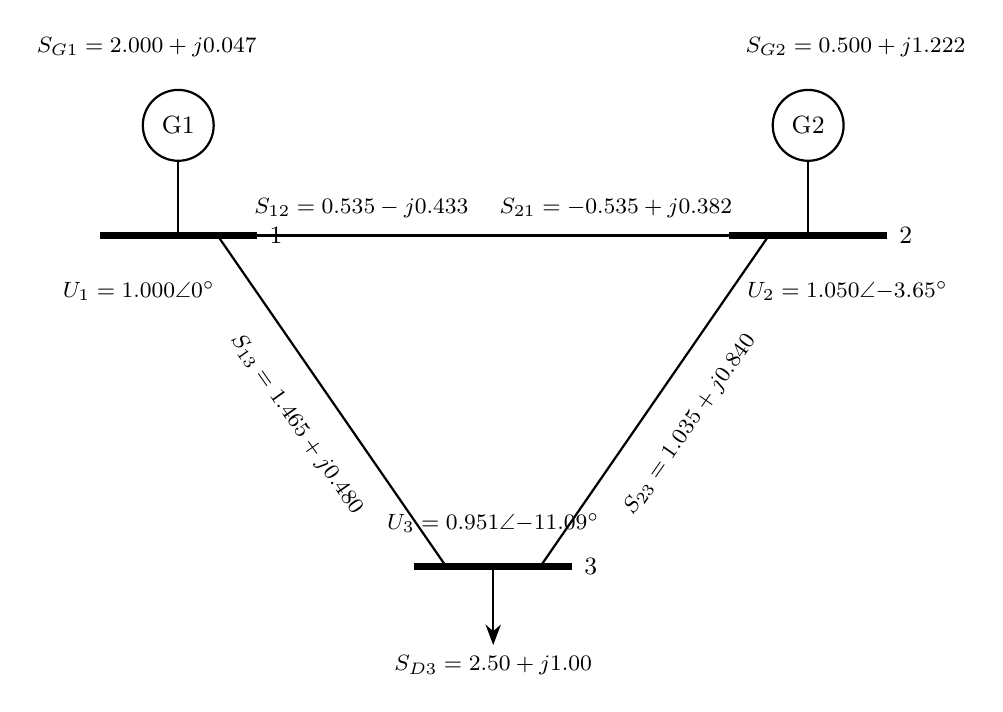
\begin{tikzpicture}[scale=1.0]
  \draw[bus] (-1.0,0) -- (1.0,0) node[right, font=\small] {1};
  \draw[bus] (7.0,0) -- (9.0,0) node[right, font=\small] {2};
  \draw[bus] (3.0,-4.2) -- (5.0,-4.2) node[right, font=\small] {3};
  \node[gen] (g1) at (0,1.4) {G1}; \draw[ln] (g1) -- (0,0);
  \node[gen] (g2) at (8,1.4) {G2}; \draw[ln] (g2) -- (8,0);
  \draw[load] (4,-4.2) -- (4,-5.2) node[below, font=\footnotesize] {$S_{D3} = 2.50 + j1.00$};
  \draw[ln] (0.8,0) -- (7.2,0) ; \draw[ln] (0.5,0) -- (3.4,-4.2); \draw[ln] (7.5,0) -- (4.6,-4.2);
  \node[lab] at (4,0.35) {$S_{12} = 0.535 - j0.433$ \quad $S_{21} = -0.535 + j0.382$};
  \node[lab, rotate=-55] at (1.5,-2.4) {$S_{13} = 1.465 + j0.480$};
  \node[lab, rotate=55] at (6.5,-2.4) {$S_{23} = 1.035 + j0.840$};
  \node[res, align=left] at (-0.5,-0.7) {$U_1 = 1.000\angle 0^\circ$};
  \node[res, align=left] at (8.5,-0.7) {$U_2 = 1.050\angle{-3.65}^\circ$};
  \node[res] at (4,-3.65) {$U_3 = 0.951\angle{-11.09}^\circ$};
  \node[font=\footnotesize, align=left] at (-0.4,2.4) {$S_{G1} = 2.000 + j0.047$};
  \node[font=\footnotesize, align=left] at (8.6,2.4) {$S_{G2} = 0.500 + j1.222$};
\end{tikzpicture}
\caption{Solved Exercise 5 (p.u.): voltages, generation and sending-end flows.}
\end{figure}

\begin{table}[h]\centering\small
\caption{Exercise 5: line flows and losses (p.u.).}
\begin{tabular}{@{}lrrr@{}}
\toprule
Line & $S_{ik}$ & $S_{ki}$ & $S_{ik,v} = S_{ik} + S_{ki}$ \\
\midrule
1-2 & $0.5352 - j0.4329$ & $-0.5352 + j0.3819$ & $0 - j0.0510$ \\
1-3 & $1.4648 + j0.4803$ & $-1.4648 - j0.2722$ & $0 + j0.2081$ \\
2-3 & $1.0352 + j0.8397$ & $-1.0352 - j0.7278$ & $0 + j0.1119$ \\
\midrule
Total & & & $S_{v,ges} = 0 + j0.2690$ \\
\bottomrule
\end{tabular}
\end{table}

\subsection{Step 7: verification}
\begin{itemize}
\item \textbf{Active balance:} $P_{G1} + P_{G2} - P_{D3} = 2.000 + 0.500 - 2.500 = 0$ = active losses (lossless lines). \checkmark
\item \textbf{Reactive balance:} $Q_{G1} + Q_{G2} - Q_{D3} = 0.047 + 1.222 - 1.000 = 0.269$ = $Q_{v,ges}$. \checkmark
\item \textbf{Independent solver:} PyPSA gives the same voltages and powers to $10^{-15}$. \checkmark
\item \textbf{Convergence:} mismatch $2.5 \to 0.21 \to 4.1\times10^{-3} \to 1.9\times10^{-6} \to 3.9\times10^{-13}$: quadratic, as expected.
\end{itemize}

\subsection{Step 8: interpretation}
The load bus sits at 0.951 p.u., just above the usual lower limit. Line 1-3 carries most of the load (1.46 p.u.).
Bus 2, held at 1.05 p.u., exports reactive power (1.22 p.u.) towards bus 3 and even towards bus 1. Line 1-2 is
lightly loaded: its charging exceeds its series losses, so its reactive ``loss'' is negative ($-j0.051$).
\begin{sayit}
``I built $\mathbf Y$ line by line, wrote three equations for three unknowns, and solved them with Newton-Raphson in
4 iterations. The slack supplies exactly 2.0 p.u.\ because the lines are lossless; all losses are reactive (0.269 p.u.).
PyPSA reproduces my result to machine precision, which validates both the model and the data conversion.''
\end{sayit}

% ================================================================ TP intro
\section{Travaux pratiques: load flow on a real network (common thread)}
\begin{gbox}{Statement (common thread of the practical work)}
We follow a case inspired by Niger: \emph{integration of a solar PV plant into a grid supplying Niamey}. Central
question: if demand grows and a solar plant is connected, do voltages stay acceptable? Can the lines carry the power?
Where do losses and congestion appear? The networks and numbers are \textbf{educational and fictitious}; they do not
represent the real Niamey grid. We go from 3 to 5, 9 and 14 buses.
\end{gbox}
\begin{figure}[h]\centering
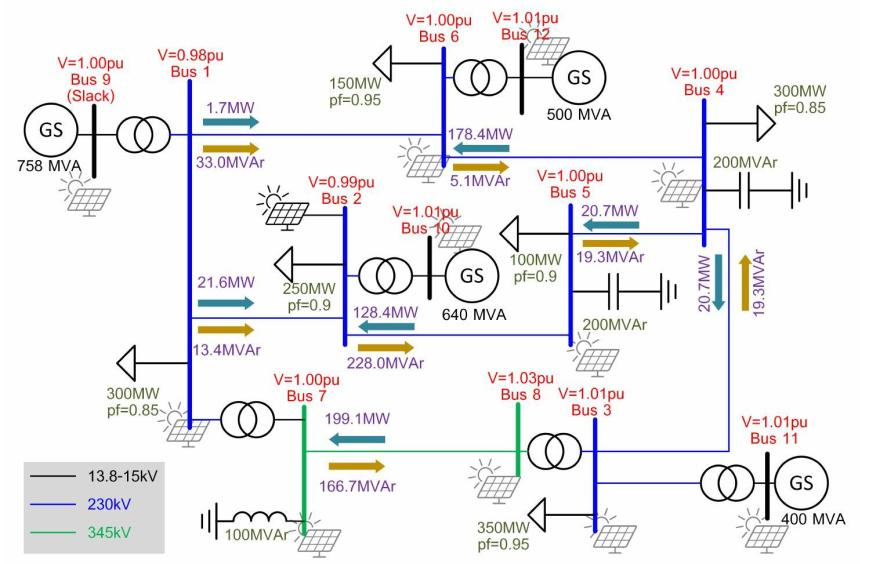
\includegraphics[width=0.72\textwidth]{tp_original_0.jpg}
\caption{Original illustration of the practical work (multi-voltage grid with solar plants).}
\end{figure}

\begin{gbox}{Simulation protocol of the practical work (applied in every TP case)}
1.~Build the network (buses, lines, transformers, generators, loads). 2.~Define the electrical parameters (nominal
voltage, $R$, $X$, thermal limits, $P$, $Q$). 3.~Define the bus types (slack, PV, PQ). 4.~Run the AC load flow.
5.~Modify the scenario (more demand, solar, set points, battery). 6.~Compare, interpret, recommend.\\[2pt]
\textbf{Indicators always reported:} $V_i$ (p.u.), $\theta_i$ ($^\circ$), $P_{ij}$ (MW), $Q_{ij}$ (MVAr), loading (\%), $P_{loss}$ (MW).
\end{gbox}

\begin{table}[h]\centering\small
\caption{Line data used in the Niamey-context cases (132 kV overhead line, ACSR 240/40 mm$^2$).}
\begin{tabular}{@{}lll@{}}
\toprule
Parameter & Value & Note \\
\midrule
$R$, $X$ & 0.12 and 0.39 $\Omega$/km & typical for 132 kV ACSR \\
$B$ (charging) & 2.9 $\mu$S/km & \\
Thermal rating & 100 MVA & hot-season value (45 $^\circ$C ambient), assumption \\
Base & $V_B = 132$ kV, $Z_B = 132^2/100 = 174.24\ \Omega$ & so 25 km: $X = 9.75\ \Omega = 0.056$ p.u. \\
\bottomrule
\end{tabular}
\end{table}

% ================================================================ TP case 1
\section{TP case 1: three-bus network, power sharing}

\subsection{Step 1: statement and question}
\begin{gbox}{Statement}
\begin{tabular}{@{}lll@{}}
Bus 1 & conventional power plant & slack bus \\
Bus 2 & city / load & 50 MW + 20 MVAr \\
Bus 3 & solar power plant & 30 MW \\
\end{tabular}\\[3pt]
The three buses are interconnected by lines. First approximation, without losses: $P_{slack} = 50 - 30 = 20$ MW.
Analyse: (1) are the voltages at buses 2 and 3 close to nominal? (2) Does the solar plant reduce the conventional
output? (3) Is there enough reactive power? (4) Are the lines adequately sized? (5) What are the total active losses?
\end{gbox}
\begin{figure}[h]\centering
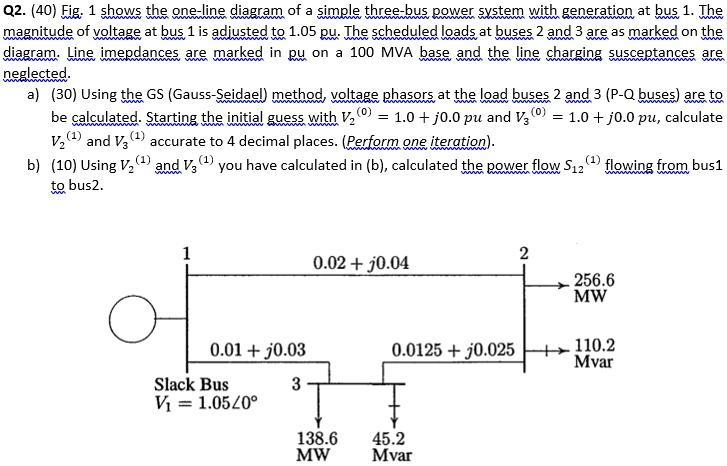
\includegraphics[width=0.62\textwidth]{tp_original_1.jpg}
\caption{Original three-bus figure of the practical work (illustration of a three-bus load-flow problem).}
\end{figure}

\subsection{Step 2: data and hypotheses}
\begin{figure}[h]\centering
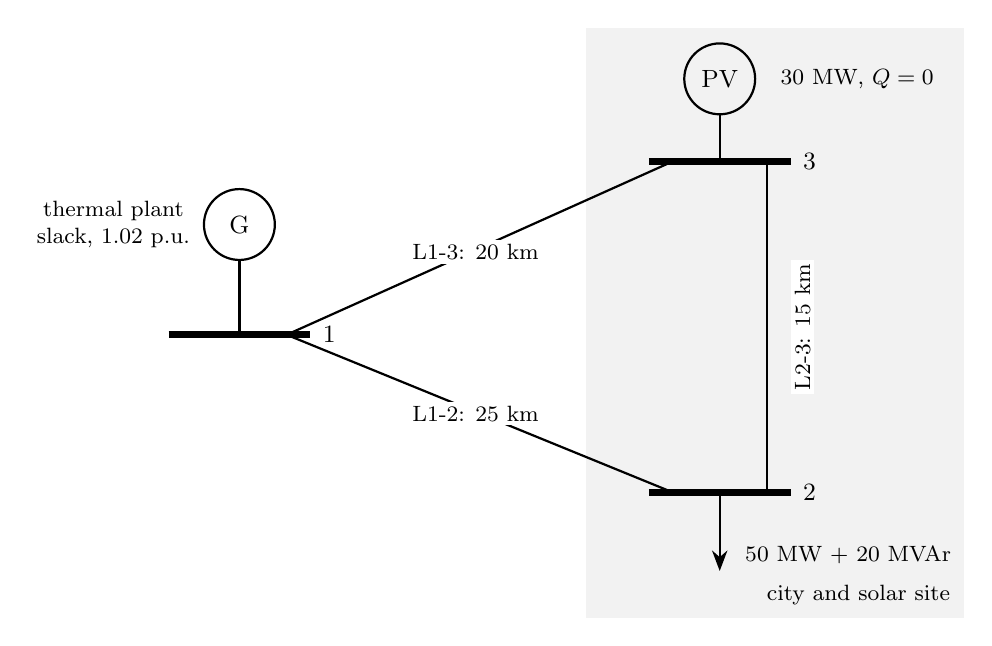
\begin{tikzpicture}
  \fill[gray!10] (4.4,-3.6) rectangle (9.2,3.9);
  \node[font=\footnotesize, anchor=south east] at (9.15,-3.55) {city and solar site};
  \draw[bus] (-0.9,0) -- (0.9,0) node[right, font=\small] {1};
  \draw[bus] (5.2,2.2) -- (7.0,2.2) node[right, font=\small] {3};
  \draw[bus] (5.2,-2.0) -- (7.0,-2.0) node[right, font=\small] {2};
  \node[gen] (g) at (0,1.4) {G}; \draw[ln] (g) -- (0,0);
  \node[font=\footnotesize, align=center] at (-1.6,1.4) {thermal plant\\slack, 1.02 p.u.};
  \node[gen] (pv) at (6.1,3.25) {PV}; \draw[ln] (pv) -- (6.1,2.2);
  \node[font=\footnotesize, align=left, anchor=west] at (6.75,3.25) {30 MW, $Q = 0$};
  \draw[load] (6.1,-2.0) -- (6.1,-3.0); \node[font=\footnotesize, anchor=west] at (6.3,-2.8) {50 MW + 20 MVAr};
  \draw[ln] (0.6,0) -- (5.5,2.2); \draw[ln] (0.6,0) -- (5.5,-2.0); \draw[ln] (6.7,-2.0) -- (6.7,2.2);
  \node[lab] at (3.0,1.05) {L1-3: 20 km};
  \node[lab] at (3.0,-1.0) {L1-2: 25 km};
  \node[lab, rotate=90] at (7.15,0.1) {L2-3: 15 km};
\end{tikzpicture}
\caption{Network modelled in PyPSA (132 kV, ratings 100 MVA).}
\end{figure}
Hypotheses: steady state, balanced three-phase, PV plant at unity power factor (PQ) unless stated, slack set point 1.02 p.u.
For question (6) of our extension, the real solar profile of 4 May 2023 (NASA POWER, Niamey, the day of the annual
demand peak) and a modelled demand shape are used.

\subsection{Step 3: model}
AC load-flow equations of section 3 for every bus; line impedances $Z = (0.12 + j0.39)\,\ell$ $\Omega$; slack
balance $P_{slack} = \sum P_{load} - P_{PV} + P_{loss}$; voltage drop $\Delta V \approx (RP + XQ)/V$.

\subsection{Step 4: method}
Three variants at the design point (no PV; PV at unity power factor; PV in voltage-control mode at 1.02 p.u.), each solved
with \texttt{n.pf()}; then 24 load flows for the real day.

\subsection{Step 5: implementation}
\code{s03_tp1_power_sharing_3bus.py}{TP case 1 in PyPSA.}

\subsection{Step 6: results}
\progout{s03.txt}{Output of Code 3.}

\begin{figure}[h]\centering
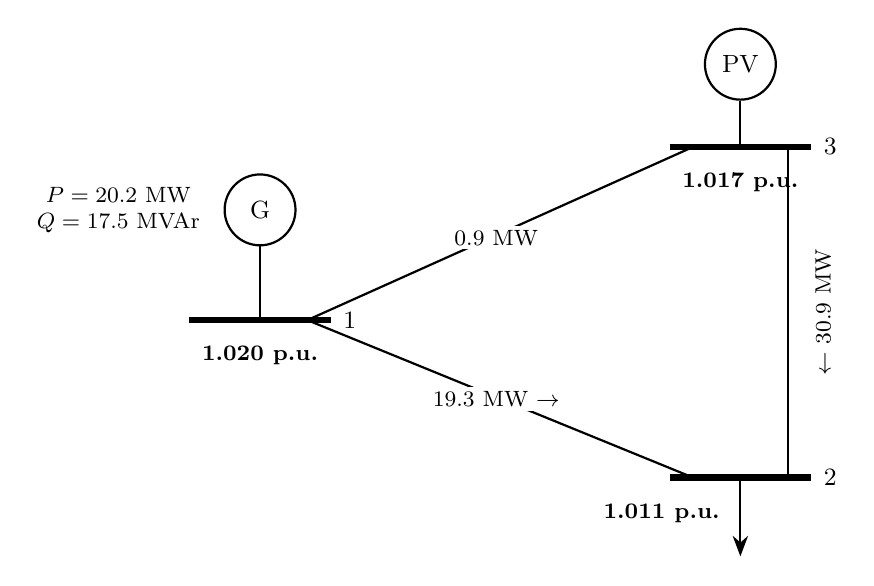
\begin{tikzpicture}
  \draw[bus] (-0.9,0) -- (0.9,0) node[right, font=\small] {1};
  \draw[bus] (5.2,2.2) -- (7.0,2.2) node[right, font=\small] {3};
  \draw[bus] (5.2,-2.0) -- (7.0,-2.0) node[right, font=\small] {2};
  \node[gen] (g) at (0,1.4) {G}; \draw[ln] (g) -- (0,0);
  \node[gen] (pv) at (6.1,3.25) {PV}; \draw[ln] (pv) -- (6.1,2.2);
  \draw[load] (6.1,-2.0) -- (6.1,-3.0);
  \draw[ln] (0.6,0) -- (5.5,2.2); \draw[ln] (0.6,0) -- (5.5,-2.0); \draw[ln] (6.7,-2.0) -- (6.7,2.2);
  \node[lab] at (3.0,1.05) {0.9 MW};
  \node[lab] at (3.0,-1.0) {19.3 MW $\rightarrow$};
  \node[lab, rotate=90] at (7.15,0.1) {$\leftarrow$ 30.9 MW};
  \node[res] at (0,-0.45) {1.020 p.u.};
  \node[res] at (6.1,1.75) {1.017 p.u.};
  \node[res] at (5.1,-2.45) {1.011 p.u.};
  \node[font=\footnotesize, align=center] at (-1.8,1.4) {$P = 20.2$ MW\\$Q = 17.5$ MVAr};
\end{tikzpicture}
\caption{Solved design point with 30 MW of PV at unity power factor: voltages and active flows.}
\end{figure}

\begin{figure}[h]\centering
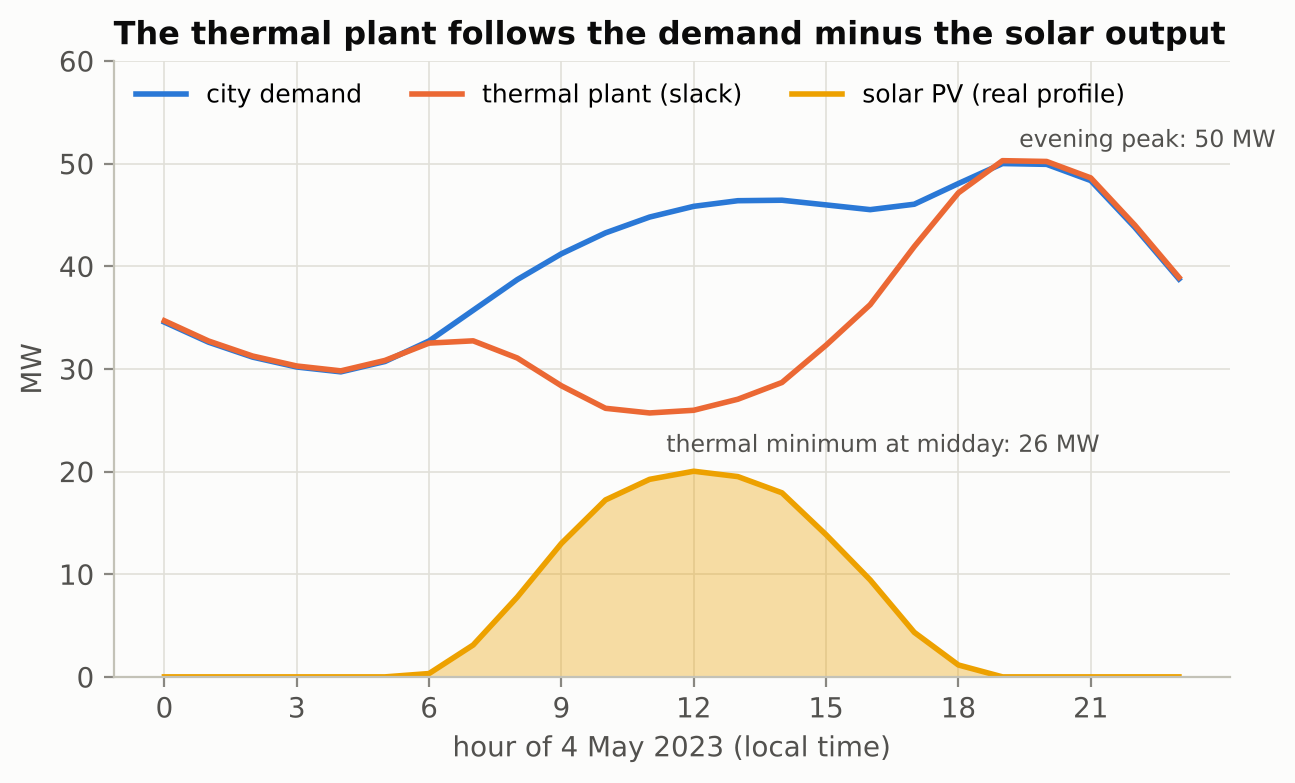
\includegraphics[width=0.72\textwidth]{cs02_day_balance.png}
\caption{Real day (4 May 2023): the thermal plant follows the demand minus the solar output.}
\end{figure}

\subsection{Step 7: verification}
Active balance with PV: $P_{slack} + P_{PV} = 20.19 + 30 = 50.19$ MW $= 50 + 0.19$ (losses). \checkmark\
Daily energy: $837.4 + 146.9 = 984.3$ MWh $= 980.3 + 4.1$ (losses). \checkmark\
Order of magnitude: on 25 km, $\Delta V \approx (3.0\cdot19.3 + 9.75\cdot10.5)/132^2 \approx 0.9\,\%$, consistent with
$1.020 \to 1.011$ p.u. \checkmark

\subsection{Step 8: interpretation}
\begin{enumerate}
\item Voltages: 1.009-1.017 p.u., close to nominal.
\item Solar reduces the thermal output from 50.3 to 20.2 MW (estimate $50 - 30 = 20$ MW, the rest is losses).
\item Reactive power: at unity PF the thermal plant gives 17.5 MVAr; in voltage control the inverters give 11.7 MVAr, below
      their 13.7 MVAr capability (33 MVA inverters at full output).
\item Lines: at most 33\,\% of the rating: adequate.
\item Losses: 0.28 MW without PV, 0.19 MW with PV (generation closer to the load).
\end{enumerate}
On the real peak day the PV plant gives at most 20 MW and 15\,\% of the energy; the peak is at 19:00, after sunset.
\begin{sayit}
``In this first case I study a three-bus grid to understand how the load is shared between conventional and solar
generation. The load flow gives the nodal voltages, the flows and the losses. Solar cuts the thermal output by 30 MW at
the design point and reduces the losses, but the evening peak stays entirely on the thermal plant.''
\end{sayit}

% ================================================================ TP case 2
\section{TP case 2: five-bus network, undervoltage}

\subsection{Step 1: statement and question}
\begin{gbox}{Statement}
\begin{tabular}{@{}lll@{}}
Bus 1 & conventional generator & slack \\
Bus 2 & substation & load 25 MW \\
Bus 3 & solar power plant & 40 MW \\
Bus 4 & urban area & 45 MW + 15 MVAr \\
Bus 5 & industrial area & 35 MW + 18 MVAr \\
\end{tabular}\\[3pt]
Bus 5 is far from generation, connected by a relatively long line. The statement \emph{assumes} the result
$V_1 = 1.00$, $V_2 = 0.99$, $V_3 = 1.01$, $V_4 = 0.97$, $V_5 = 0.92$ p.u.\ (illustrative values, not a simulation) and asks
which problem is solved (undervoltage, limit 0.95 p.u.) and which solutions an engineer can study.
\end{gbox}
\begin{figure}[h]\centering
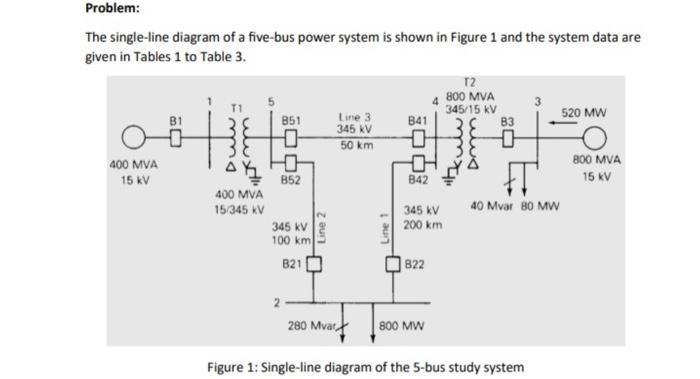
\includegraphics[width=0.58\textwidth]{tp_original_2.jpg}
\caption{Original five-bus figure of the practical work.}
\end{figure}

\subsection{Step 2: data and hypotheses}
\begin{figure}[h]\centering
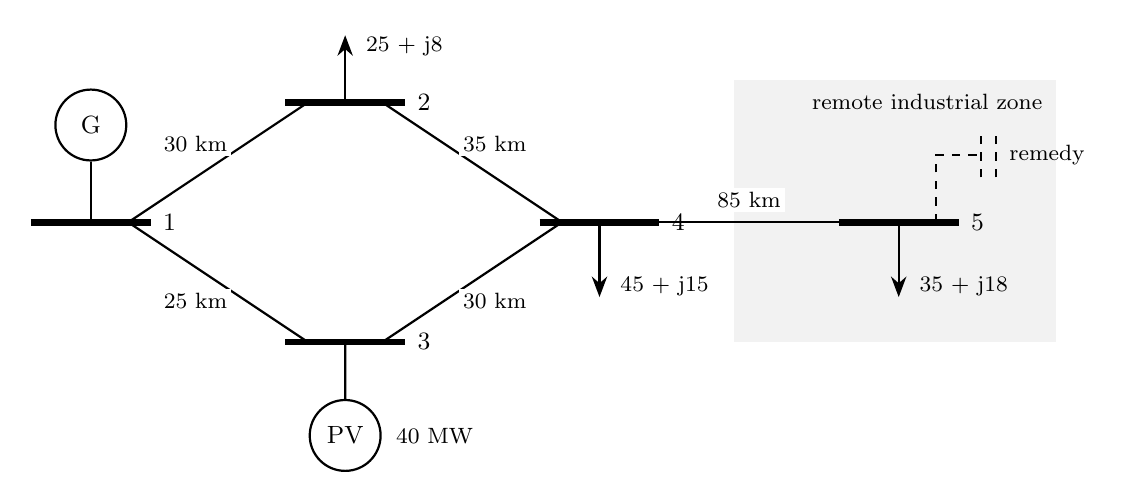
\begin{tikzpicture}[scale=0.95]
  \fill[gray!10] (8.6,-1.6) rectangle (12.9,1.9);
  \node[font=\footnotesize, anchor=north east] at (12.85,1.85) {remote industrial zone};
  \draw[bus] (-0.8,0) -- (0.8,0) node[right, font=\small] {1};
  \draw[bus] (2.6,1.6) -- (4.2,1.6) node[right, font=\small] {2};
  \draw[bus] (2.6,-1.6) -- (4.2,-1.6) node[right, font=\small] {3};
  \draw[bus] (6.0,0) -- (7.6,0) node[right, font=\small] {4};
  \draw[bus] (10.0,0) -- (11.6,0) node[right, font=\small] {5};
  \node[gen] (g) at (0,1.3) {G}; \draw[ln] (g) -- (0,0);
  \node[gen] (pv) at (3.4,-2.85) {PV}; \draw[ln] (pv) -- (3.4,-1.6);
  \node[font=\footnotesize, anchor=west] at (3.95,-2.85) {40 MW};
  \draw[load] (3.4,1.6) -- (3.4,2.5); \node[font=\footnotesize, anchor=west] at (3.55,2.35) {25 + j8};
  \draw[load] (6.8,0) -- (6.8,-1.0); \node[font=\footnotesize, anchor=west] at (6.95,-0.85) {45 + j15};
  \draw[load] (10.8,0) -- (10.8,-1.0); \node[font=\footnotesize, anchor=west] at (10.95,-0.85) {35 + j18};
  \draw[ln] (0.5,0) -- (2.9,1.6); \draw[ln] (0.5,0) -- (2.9,-1.6);
  \draw[ln] (3.9,1.6) -- (6.3,0); \draw[ln] (3.9,-1.6) -- (6.3,0);
  \draw[ln] (7.3,0) -- (10.3,0);
  \node[lab] at (1.4,1.05) {30 km}; \node[lab] at (1.4,-1.05) {25 km};
  \node[lab] at (5.4,1.05) {35 km}; \node[lab] at (5.4,-1.05) {30 km};
  \node[lab] at (8.8,0.3) {85 km};
  \draw[ln, dashed] (11.3,0) -- (11.3,0.9) -- (11.9,0.9);
  \draw[ln, dashed] (11.9,0.6) -- (11.9,1.2); \draw[ln, dashed] (12.1,0.6) -- (12.1,1.2);
  \node[font=\footnotesize, anchor=west] at (12.15,0.9) {remedy};
\end{tikzpicture}
\caption{Network modelled in PyPSA (132 kV). Loads in MW + jMVAr; dashed: capacitor bank studied as remedy.}
\end{figure}
Hypotheses: same line data as case 1; slack 1.02 p.u.; the statement leaves the length free: 85 km is chosen so that the
\emph{computed} $V_5$ matches the order of magnitude of the statement (0.92 p.u.); substation load 25 MW + 8 MVAr
(power factor 0.95, assumption). Two design points: A = statement (PV at 40 MW); B = evening peak, no sun.

\subsection{Step 3: model}
\[ \Delta V_{4\to5} \approx \frac{R P + X Q}{V}, \qquad R = 0.12\cdot85 = 10.2\ \Omega,\quad X = 0.39\cdot85 = 33.2\ \Omega. \]
$X \approx 3R$: each MVAr transported costs three times more voltage than each MW. A capacitor bank $Q_c$ at bus 5
produces $Q_c V^2$ locally and removes that reactive flow from the line.

\subsection{Step 4: method}
(1) AC load flow for A and B. (2) Five remedies at the worst case. (3) Smallest capacitor by bisection on $V_5 \ge 0.95$.
(4) The real day with and without the bank.

\subsection{Step 5: implementation}
\code{s04_tp2_undervoltage_5bus.py}{TP case 2 in PyPSA.}

\subsection{Step 6: results}
\progout{s04.txt}{Output of Code 4.}

\begin{figure}[h]\centering
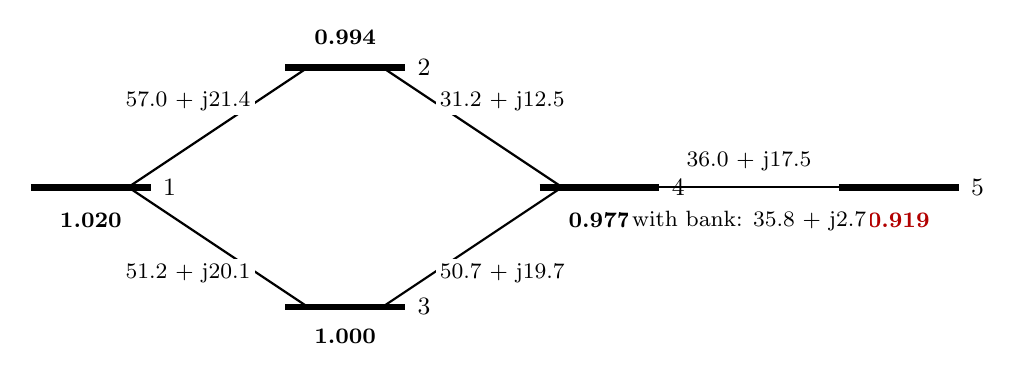
\begin{tikzpicture}[scale=0.95]
  \draw[bus] (-0.8,0) -- (0.8,0) node[right, font=\small] {1};
  \draw[bus] (2.6,1.6) -- (4.2,1.6) node[right, font=\small] {2};
  \draw[bus] (2.6,-1.6) -- (4.2,-1.6) node[right, font=\small] {3};
  \draw[bus] (6.0,0) -- (7.6,0) node[right, font=\small] {4};
  \draw[bus] (10.0,0) -- (11.6,0) node[right, font=\small] {5};
  \draw[ln] (0.5,0) -- (2.9,1.6); \draw[ln] (0.5,0) -- (2.9,-1.6);
  \draw[ln] (3.9,1.6) -- (6.3,0); \draw[ln] (3.9,-1.6) -- (6.3,0); \draw[ln] (7.3,0) -- (10.3,0);
  \node[res] at (0,-0.45) {1.020}; \node[res] at (3.4,2.0) {0.994}; \node[res] at (3.4,-2.0) {1.000};
  \node[res] at (6.8,-0.45) {0.977}; \node[res] at (10.8,-0.45) {\color{red!70!black}0.919};
  \node[lab] at (1.3,1.15) {57.0 + j21.4}; \node[lab] at (1.3,-1.15) {51.2 + j20.1};
  \node[lab] at (5.5,1.15) {31.2 + j12.5}; \node[lab] at (5.5,-1.15) {50.7 + j19.7};
  \node[lab] at (8.8,0.35) {36.0 + j17.5}; \node[lab] at (8.8,-0.45) {with bank: 35.8 + j2.7};
\end{tikzpicture}
\caption{Solved worst case B (evening peak, no PV): voltages (p.u.) and sending-end flows (MW + jMVAr).
With the 15 MVAr bank, the reactive flow on line 4-5 falls from 17.5 to 2.7 MVAr and $V_5$ rises to 0.959 p.u.}
\end{figure}

\begin{figure}[h]\centering
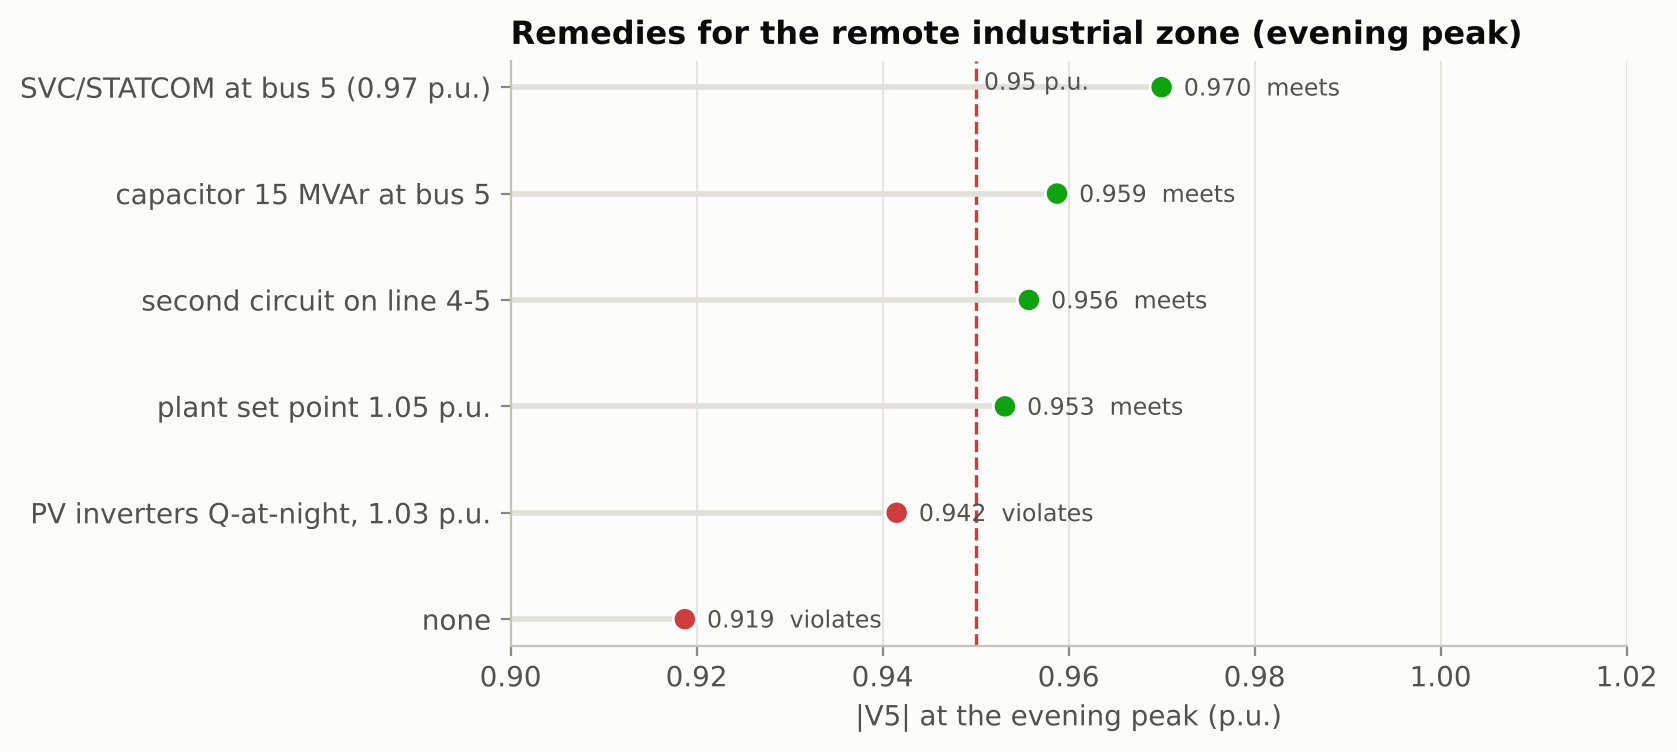
\includegraphics[width=0.68\textwidth]{cs03_remedies.png}
\caption{The five remedies at the evening peak.}
\end{figure}

\subsection{Step 7: verification}
Hand estimate on line 4-5 (case B): $\Delta V \approx (10.2\cdot36.0 + 33.2\cdot17.5)/132^2 = 5.4\,\%$; computed drop
$0.977 - 0.919 = 5.8\,\%$ (the difference is the $I^2X$ term and the voltage level). \checkmark\
Sensitivity: about 3.6 MVAr per percent of voltage at bus 5, so 11.8 MVAr for the missing 3.1 points. \checkmark

\subsection{Step 8: interpretation}
Only bus 5 is out of limits, 24 hours a day: the problem is \textbf{structural} (distance and reactive demand), not a peak
accident. The PV plant does not help (far away, no sun at the peak; its inverters would need 68 MVAr, more than their
44 MVA). \textbf{Recommendation:} a 15 MVAr switched capacitor bank (3 $\times$ 5 MVAr) at bus 5; cheapest, it also cuts
losses by 14\,\% at the peak; keep a second circuit as the long-term option.
\begin{sayit}
``In the five-bus network the problem is localised: bus 5 falls to 0.92 p.u.\ because it is fed through a long line and
its load is strongly reactive. I compared five remedies with the load flow; a 15 MVAr capacitor bank restores
0.96 p.u.\ all day and reduces the losses.''
\end{sayit}

% ================================================================ TP case 3
\section{TP case 3: IEEE 9-bus system, congestion}

\subsection{Step 1: statement and question}
\begin{gbox}{Statement}
Reference IEEE 9-bus system: several generators, several loads, interconnected lines. New problem: line congestion.
\emph{Suppose a line has a thermal limit of 100 MVA and carries 115 MVA after the load flow: loading 115\,\%}
(illustrative). Solutions to study: redispatch of generation, line reinforcement, topology change, new link, storage.
\end{gbox}
\begin{figure}[h]\centering
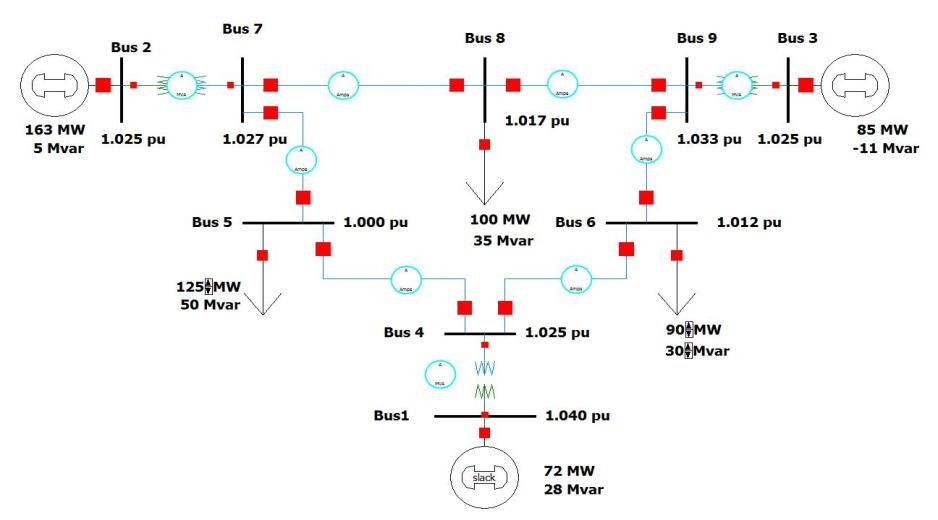
\includegraphics[width=0.62\textwidth]{tp_original_3.jpg}
\caption{Original IEEE 9-bus figure of the practical work.}
\end{figure}

\subsection{Step 2: data and hypotheses}
Official MATPOWER data \texttt{case9.m} (written out in Code 5): 345 kV, 100 MVA base, ratings 150-300 MVA, quadratic
generator costs. To create the congestion with a physical cause (instead of an arbitrary 100 MVA): hot-season ratings
15\,\% below the MATPOWER values, and an evening peak 15\,\% above the base load. Security criterion N-1: every single
line outage must leave all other lines within their rating.

\subsection{Step 3: model}
Economic dispatch (DC optimal power flow): $\min \sum_g (c_{2,g}P_g^2 + c_{1,g}P_g)$ s.t.\ nodal balance and
$|P_\ell| \le s_{nom,\ell}$. Security-constrained OPF: the same with the post-outage flows
$P_\ell + \text{LODF}_{\ell c}\,P_c \le s_{nom,\ell}$ for every outage $c$. The locational marginal price (LMP) is the
dual variable of the nodal balance.

\subsection{Step 4: method}
(1) Economic dispatch. (2) AC check of the intact grid. (3) AC N-1 screening. (4) Security-constrained OPF and new AC
screening. (5) Reactive support sized by bisection for the voltage problem found. (6) Reinforcement option.

\subsection{Step 5: implementation}
\code{s05_tp3_congestion_ieee9.py}{TP case 3 in PyPSA.}

\subsection{Step 6: results}
\progout{s05.txt}{Output of Code 5.}
\begin{figure}[h]\centering
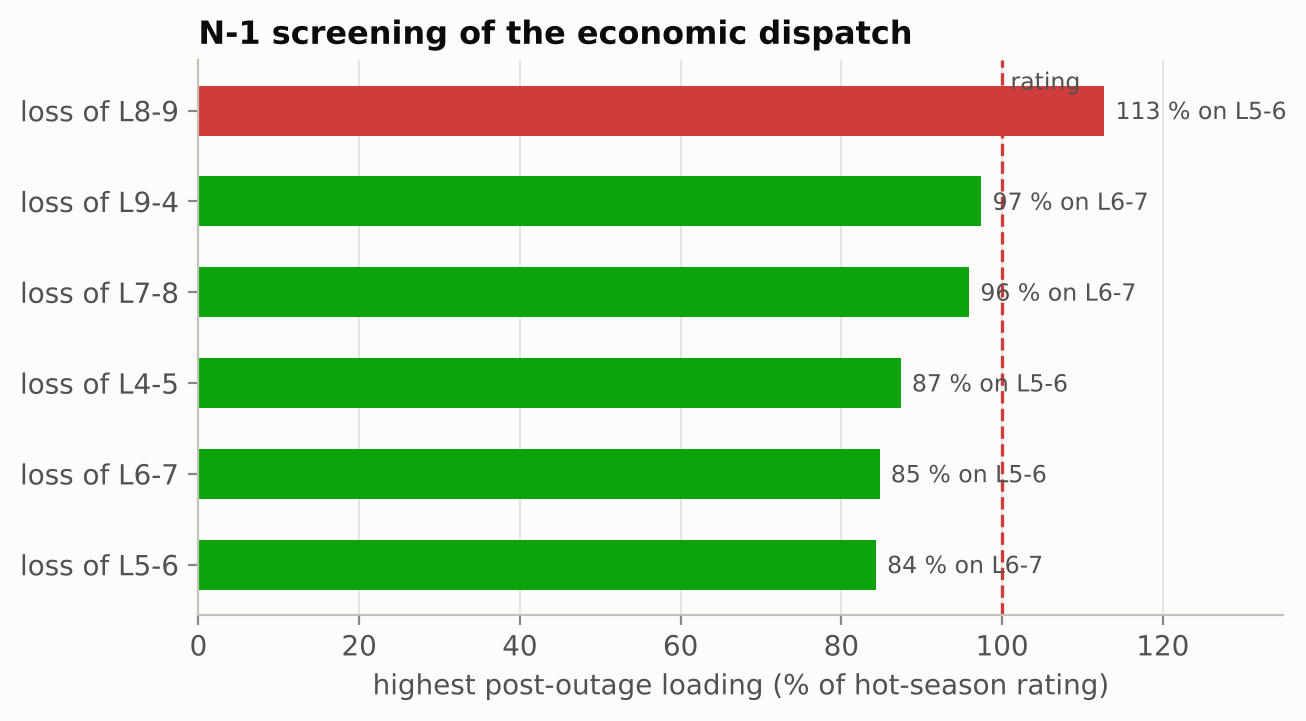
\includegraphics[width=0.49\textwidth]{cs04_n1_economic.png}\hfill
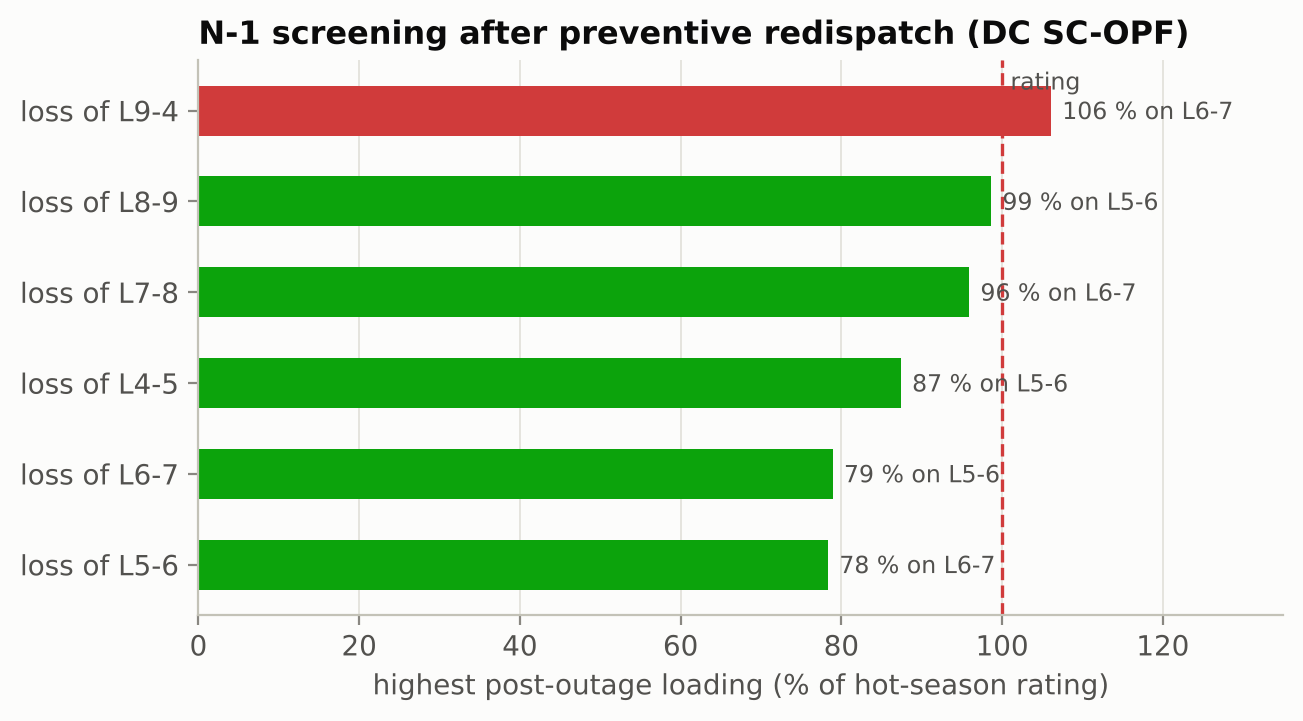
\includegraphics[width=0.49\textwidth]{cs04_n1_secure.png}
\caption{Worst post-outage loading: economic dispatch (left) and secure dispatch (right).}
\end{figure}

\subsection{Step 7: verification}
Generation $101.4 + 153.5 + 107.3 = 362.2$ MW $= 1.15 \times 315$ MW (DC model, no losses). \checkmark\
The DC security constraint is re-checked with the full AC model: line 5-6 at 98.7\,\% after the loss of 8-9. \checkmark\
The AC check also reveals what the DC model cannot see (next step).

\subsection{Step 8: interpretation}
The cheapest dispatch is not N-1 secure: losing line 8-9 overloads line 5-6 to \textbf{113\,\%} (close to the 115\,\% of
the statement, but computed). Preventive redispatch (18 MW moved from G2/G3 to G1) removes it for \textbf{54 \$/h}
(0.8\,\%); nodal prices separate (25.5 to 31.3 \$/MWh). The AC check finds a second, hidden problem: losing line 9-4
drops bus 9 to 0.75 p.u.\ and overloads line 6-7 (106\,\%); \textbf{62 MVAr} of switched reactive support at bus 9 cures
both. Uprating line 5-6 removes the flow problem but not the voltage problem.
\begin{sayit}
``The IEEE 9-bus system shows that a line can exceed its capacity after an outage. I evaluated redispatch,
reinforcement and reactive support. Redispatch costs less than 1\,\% and is the right first answer; the AC check proved
that a voltage reserve at bus 9 is also needed.''
\end{sayit}

% ================================================================ TP case 4
\section{TP case 4: IEEE 14-bus system, demand growth}

\subsection{Step 1: statement and question}
\begin{gbox}{Statement}
Reference IEEE 14-bus system (14 nodes, generators, loads, transformers, lines). Demand grows: S0 = 100\,\%, S1 = 110\,\%,
S2 = 120\,\%, S3 = 130\,\%. For each scenario compare: (1) minimum voltage, (2) number of buses in undervoltage,
(3) maximum line loading, (4) active losses, (5) reactive power supplied by the generators. The statement gives an
\emph{illustrative} table (e.g.\ S3: 0.90 p.u., 112\,\%, 8.0 MW, 4 buses below 0.95).
\end{gbox}
\begin{figure}[h]\centering
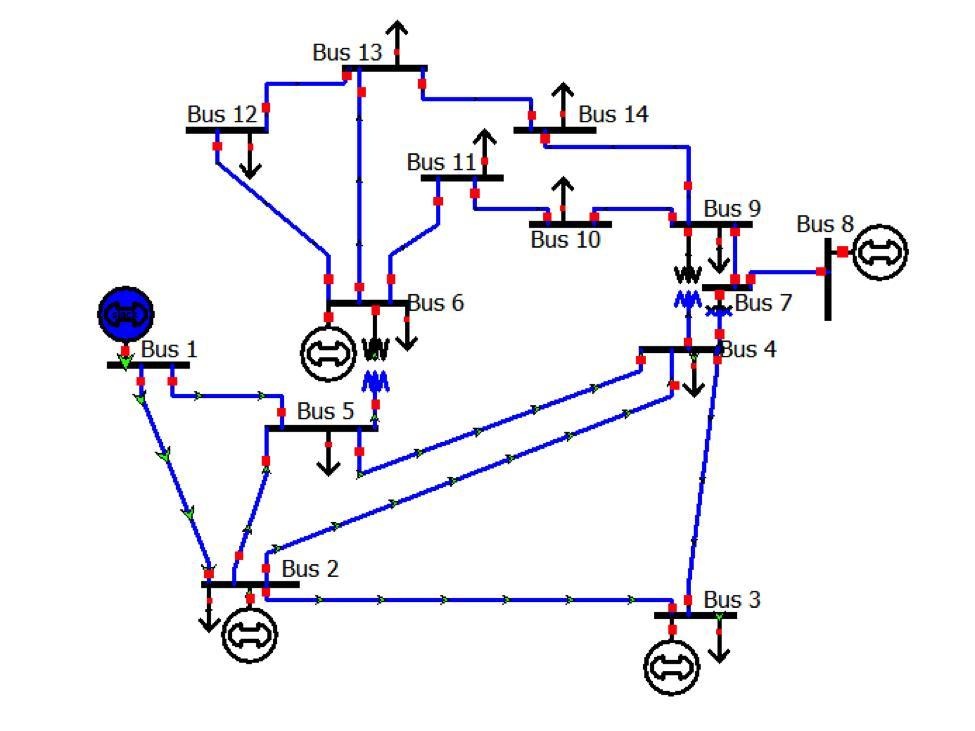
\includegraphics[width=0.5\textwidth]{tp_original_4.jpg}
\caption{Original IEEE 14-bus figure of the practical work.}
\end{figure}

\subsection{Step 2: data and hypotheses}
Official MATPOWER \texttt{case14.m} (dataset \texttt{data/networks/ieee14}); thermal ratings from the IEEE PES benchmark
PGLib-OPF; generator reactive limits from MATPOWER (G1 0-10, G2 $-40$/50, G3 0/40, G6 and G8 $-6$/24 MVAr). All loads
scale with the same factor; G2 follows, the slack takes the rest. Hypothesis: reactive limits \textbf{are enforced}.

\subsection{Step 3: model}
AC load flow plus reactive limits: a PV generator with $Q > Q_{max}$ becomes PQ at $Q_{max}$ (PV $\to$ PQ switching); its
bus voltage is then free. Beyond the maximum loadability the Jacobian is singular and no solution exists.

\subsection{Step 4: method}
Load flow with PV $\to$ PQ switching for S0 to S5; same scenarios without limits for comparison; increase the load in
steps of 1\,\% until the load flow has no solution (maximum loadability).

\subsection{Step 5: implementation}
\code{s06_tp4_demand_growth_ieee14.py}{TP case 4 in PyPSA.}

\subsection{Step 6: results}
\progout{s06.txt}{Output of Code 6.}
\begin{figure}[h]\centering
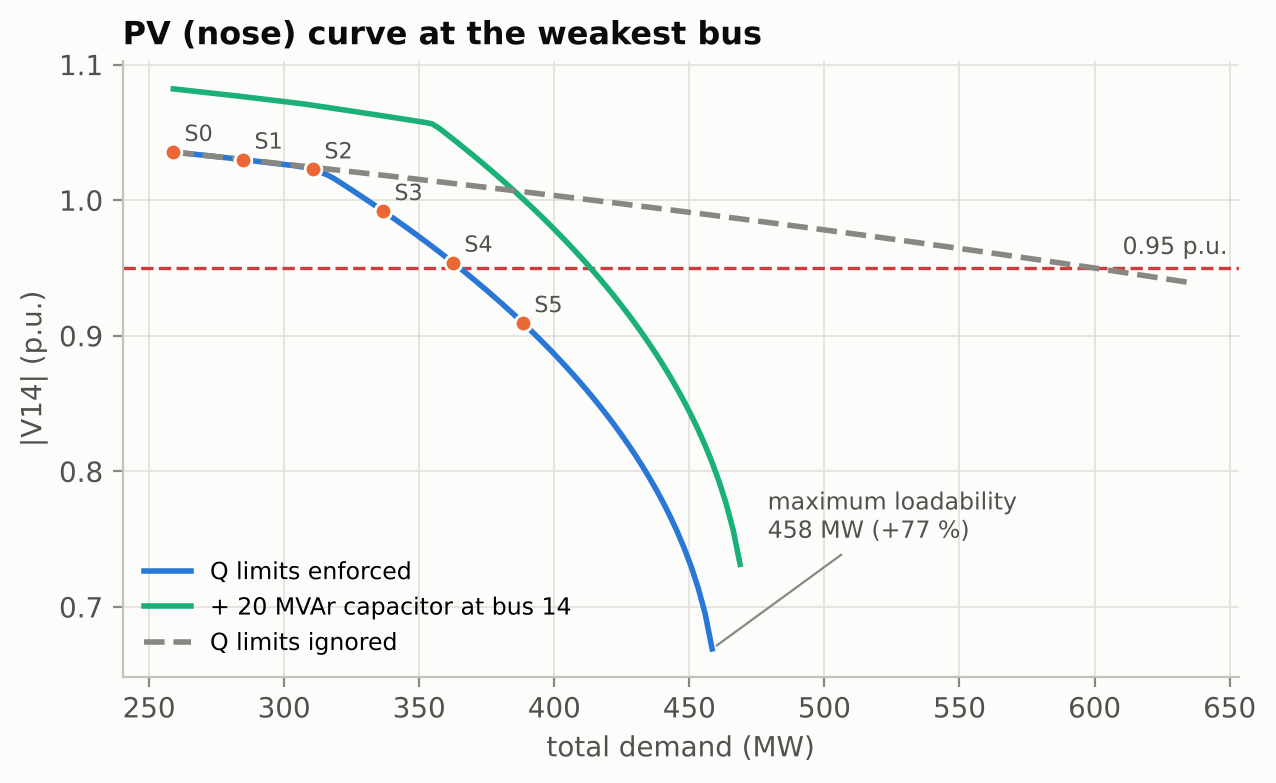
\includegraphics[width=0.66\textwidth]{cs05_pv_curve.png}
\caption{PV (nose) curve at bus 14: S0 to S5 and the maximum loadability.}
\end{figure}

\subsection{Step 7: verification}
S0 reproduces the published IEEE 14-bus solution (slack 232.4 MW, losses 13.393 MW) and our own Newton-Raphson solver
to $10^{-13}$. \checkmark\ Losses grow faster than demand ($\times 2.6$ for $\times 1.5$): consistent with $I^2R$. \checkmark

\subsection{Step 8: interpretation}
Up to +30\,\% the indicators look healthy (min 0.983 p.u., no line above 79\,\%), yet the four voltage-control units are all
at their reactive limit: \textbf{the reactive reserve runs out first}. At +50\,\% nine buses fall below 0.95 p.u. The
maximum loadability is +77\,\%; ignoring reactive limits (the default behaviour) would wrongly suggest more than +145\,\%.
\begin{sayit}
``I studied the sensitivity of the IEEE 14-bus network to demand growth. Voltages decrease, losses and line loadings
increase, and the reactive reserve is exhausted at +30\,\%. Beyond about +40\,\% operating limits are violated:
reactive compensation and reinforcement must be planned before that point.''
\end{sayit}

% ================================================================ TP case 5
\section{TP case 5: solar plant in the 14-bus network, reverse flow and storage}

\subsection{Step 1: statement and question}
\begin{gbox}{Statement}
Scenarios: S0 no solar; S1 50 MW of solar; S2 100 MW of solar; S3 100 MW of solar + storage. Solar integration can
reverse flows, raise voltages locally, reduce conventional output and change reactive needs. \emph{Example: a substation
receives 40 MW; a local plant produces 60 MW while the local load stays at 40 MW: the surplus $60 - 40 = 20$ MW flows
back upstream.} A battery does not automatically solve voltage or congestion problems: its location, power, energy and
control strategy must be studied.
\end{gbox}
\begin{figure}[h]\centering
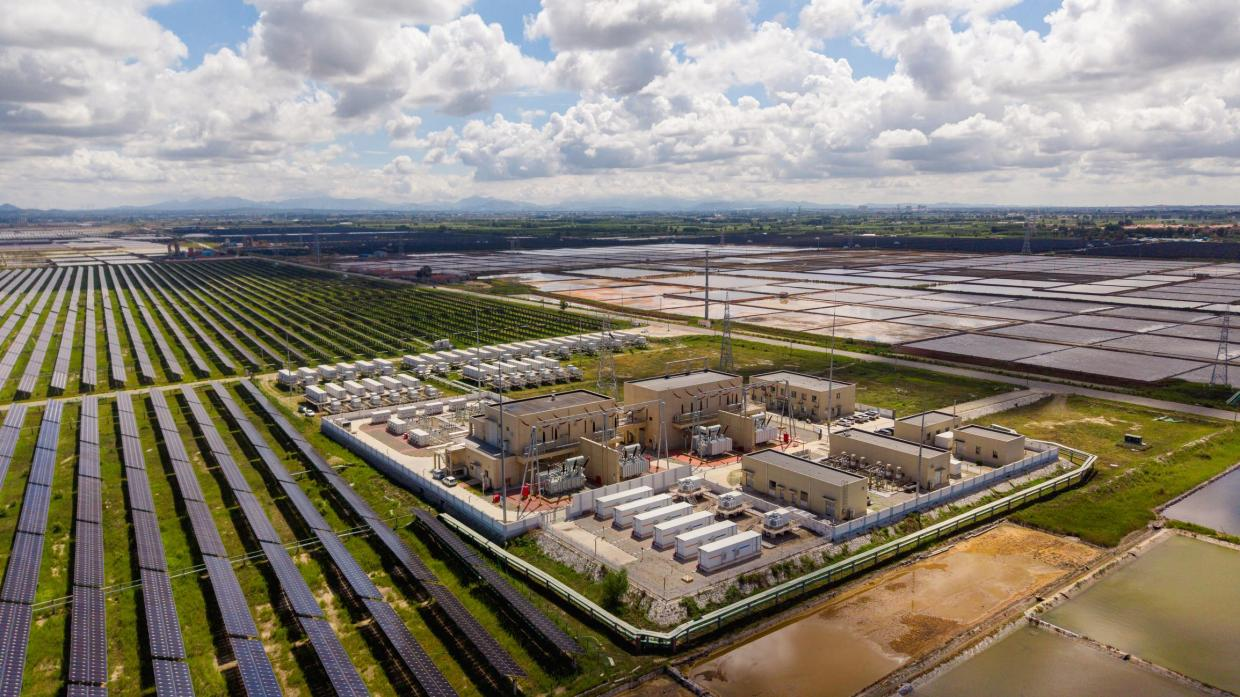
\includegraphics[width=0.5\textwidth]{tp_original_5.jpg}
\caption{Original illustration: solar plant with battery storage.}
\end{figure}

\subsection{Step 2: data and hypotheses}
IEEE 14-bus (case 4) with the plant at \textbf{bus 14}, the weakest node (local load about 14 MW at noon). Real solar
profile of 16 March 2023 (clearest day of the first quarter, Niamey). Battery 50 MW / 200 MWh at bus 14. Voltage limits
0.94-1.06 p.u.\ on the customer buses (generator buses are held at their set points; bus 7 is a transformer star point).

\subsection{Step 3: model}
Reverse flow: $P_{surplus} = P_{PV} - P_{load}$ leaves the node. Voltage rise: $\Delta V \approx (RP + XQ)/V$ with $P$ now
exported; absorbing reactive power ($Q < 0$, PF 0.95: $Q = -0.33P$) compensates it. Hosting capacity: the largest PV
power before the first limit is violated.

\subsection{Step 4: method}
(1) Hosting capacity at noon for three strategies (1 MW steps). (2) Flows into bus 14 versus PV size. (3) The four
scenarios of the statement plus S4 = S3 + reactive control + lower set points, over 24 hours. Battery rule: peak shaving
(store the PV above the lowest threshold that fills 200 MWh; return it 18:00-22:00).

\subsection{Step 5: implementation}
\code{s07_tp5_solar_storage_ieee14.py}{TP case 5 in PyPSA.}

\subsection{Step 6: results}
\progout{s07.txt}{Output of Code 7.}
\begin{figure}[h]\centering
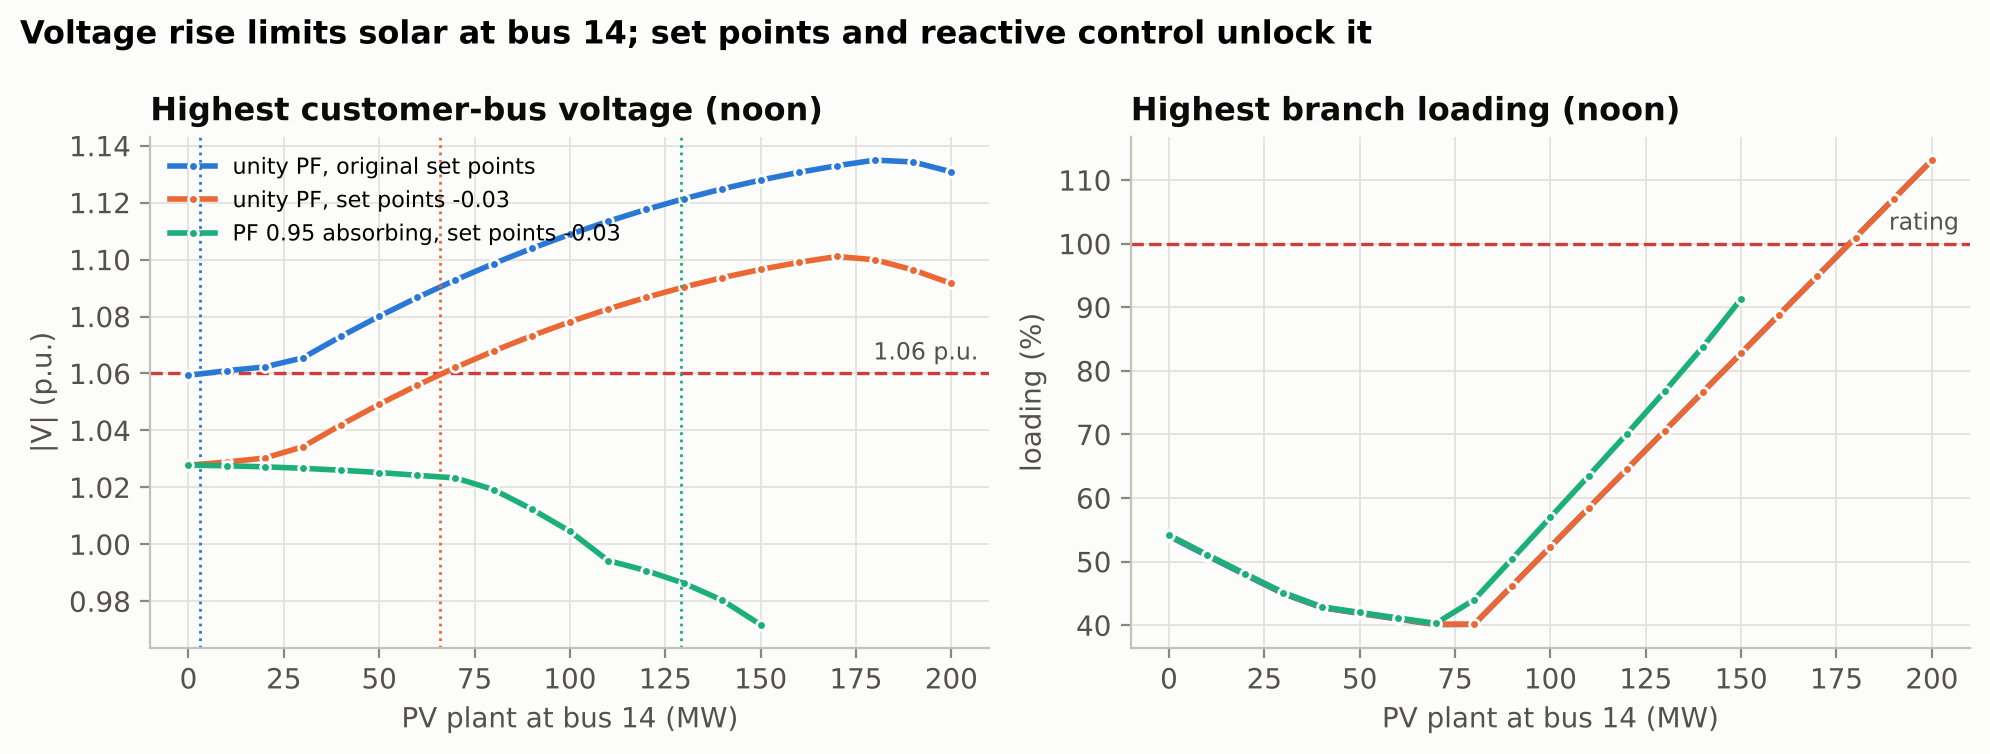
\includegraphics[width=0.95\textwidth]{cs06_hosting_capacity.png}
\caption{Hosting capacity of bus 14 at noon: voltage, not line capacity, is the limit.}
\end{figure}
\begin{figure}[h]\centering
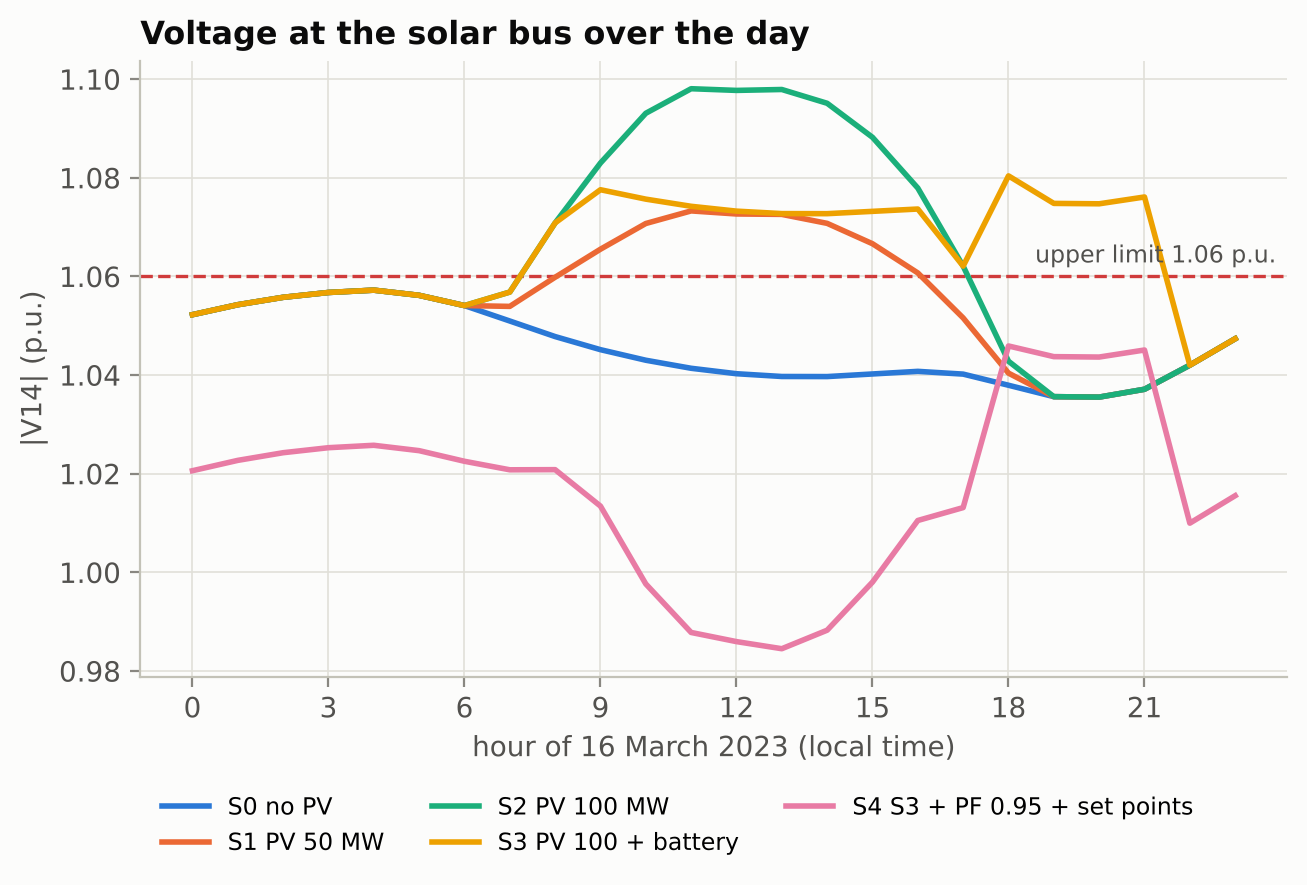
\includegraphics[width=0.66\textwidth]{cs06_day_v14.png}
\caption{Voltage at the solar bus over the day for the five scenarios.}
\end{figure}

\subsection{Step 7: verification}
Reverse flow appears between 10 and 14 MW of PV: exactly where PV equals the local noon load (13.8 MW), as the
statement's formula $P_{surplus} = P_{PV} - P_{load}$ predicts. \checkmark\ With 100 MW the export is 81.8 MW at noon
$\approx 100 - 13.8 - $ losses. \checkmark

\subsection{Step 8: interpretation}
The original voltage set points leave almost no margin (hosting capacity 3 MW). Lowering the set points by 0.03 p.u.\
(free) gives 66 MW; adding inverter reactive control gives 129 MW. The battery reduces the peak voltage
(1.098 $\to$ 1.080 p.u.) and the export (62 $\to$ 37 MW), but its evening discharge at the weak node raises the voltage
there: \textbf{storage needs a voltage-aware strategy}. The full package (S4) removes every overvoltage hour.
\begin{sayit}
``Solar changes where power is injected. When local production exceeds local demand the flow reverses, and the voltage
rises. I measured the hosting capacity and showed that set points and inverter reactive control increase it from 3 to
129 MW; the battery helps only with the right location and control.''
\end{sayit}

% ================================================================ real case A
\section{Real case A: solar and storage for the Niamey area, every hour of 2023}

\subsection{Step 1: statement and question}
\begin{gbox}{Statement (decision case)}
The Niamey area is supplied by a thermal plant (HFO/diesel, fuel 180 \$/MWh) and by imports (70 \$/MWh), which can be
interrupted (as in 2023). How much solar and battery capacity minimises the yearly cost of supply, with and without
imports? What does it change for fuel, CO$_2$ and the grid? Six scenarios (``islanded'' = imports interrupted): A imports, no PV; B no imports, no PV;
C no imports, 100 MW of PV; D0 no imports, optimal PV only; D no imports, optimal PV + battery; E imports, optimal PV + battery.
\end{gbox}

\subsection{Step 2: data and hypotheses}
\begin{table}[h]\centering\small
\caption{Real case A: data (dataset \texttt{data/networks/niamey\_grid\_2023}).}
\begin{tabularx}{\textwidth}{@{}l>{\raggedright\arraybackslash}X>{\raggedright\arraybackslash}p{3.6cm}@{}}
\toprule
Item & Value & Source / status \\
\midrule
Weather & hourly 2023, irradiance and temperature, Niamey & NASA POWER (real) \\
PV output & pvlib: Hay-Davies, Faiman, PVWatts, 10\,\% losses; 1\,710 kWh/kWp & same chain as Renewables.ninja \\
Demand & 726 GWh, peak 105 MW, temperature-driven & model (assumption) \\
Grid & five-bus network of TP case 2 + 15 MVAr bank & fictitious \\
PV cost & 800 \$/kW, 25 years, 8\,\% $\Rightarrow$ 86.9 k\$/MW/yr & IRENA (2024) range \\
Battery & 4 h, 1\,150 \$/kW, 15 years $\Rightarrow$ 157.4 k\$/MW/yr; 90\,\% round trip & NREL ATB range \\
Islanded operation & thermal must-run 20 MW (inertia, frequency control) & assumption \\
\bottomrule
\end{tabularx}
\end{table}

\subsection{Step 3: model}
Linear optimal power flow with investment over the 8760 hours:
\[ \min\; \sum_{a\in\{PV,\,bat\}} c^{cap}_a \bar P_a + \sum_t \sum_g c_g\, p_{g,t} \]
subject to nodal balance every hour, $|P_{\ell,t}| \le 0.9\,s_{nom}$, $p_{PV,t} \le \bar P_{PV}\,CF_t$, battery state of
charge $e_{t} = e_{t-1} + 0.95\,p^{ch}_t - p^{dis}_t/0.95$, $0 \le e_t \le 4\bar P_{bat}$, and the must-run when islanded.

\subsection{Step 4: method}
Solve the six scenarios with \texttt{n.optimize()} (HiGHS); then take the optimal hourly dispatch of D and run the full AC
load flow at the two critical hours (evening peak, solar peak).

\subsection{Step 5: implementation}
\code{s08_real_case_niamey.py}{Real case A in PyPSA.}

\subsection{Step 6: results}
\progout{s08.txt}{Output of Code 8.}
\begin{figure}[h]\centering
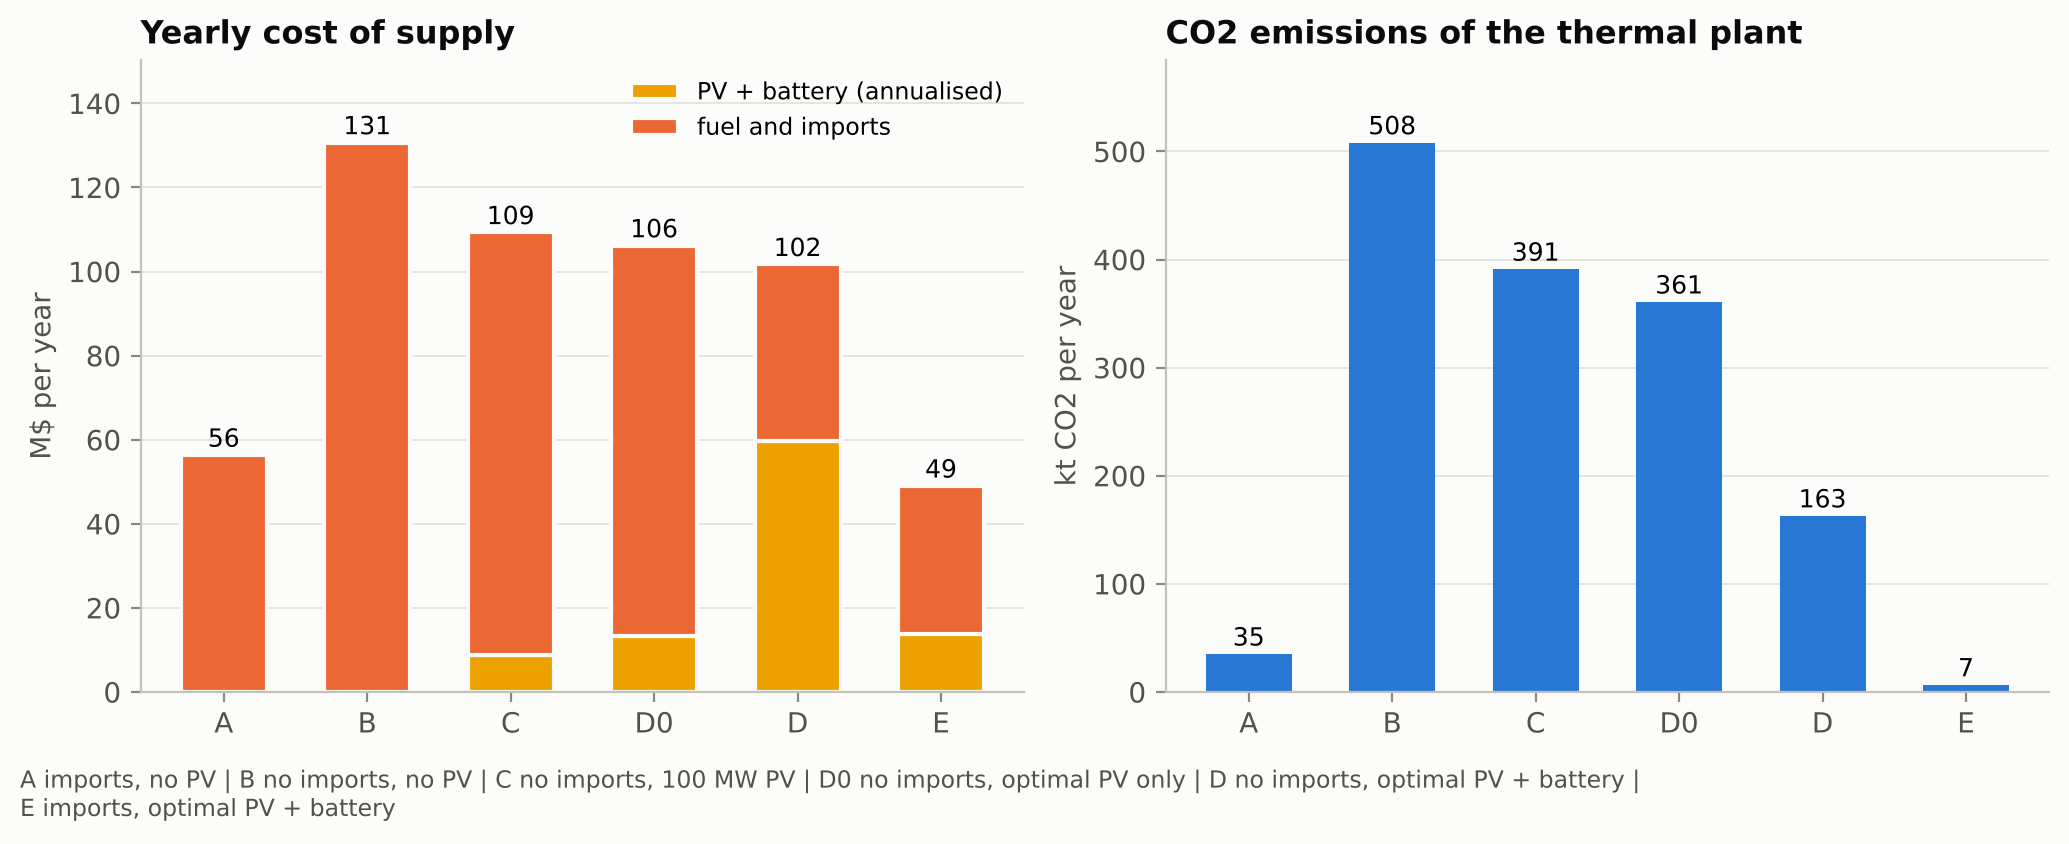
\includegraphics[width=0.95\textwidth]{cs07_cost_co2.png}
\caption{Yearly cost of supply and CO$_2$ emissions of the six scenarios.}
\end{figure}
\begin{figure}[h]\centering
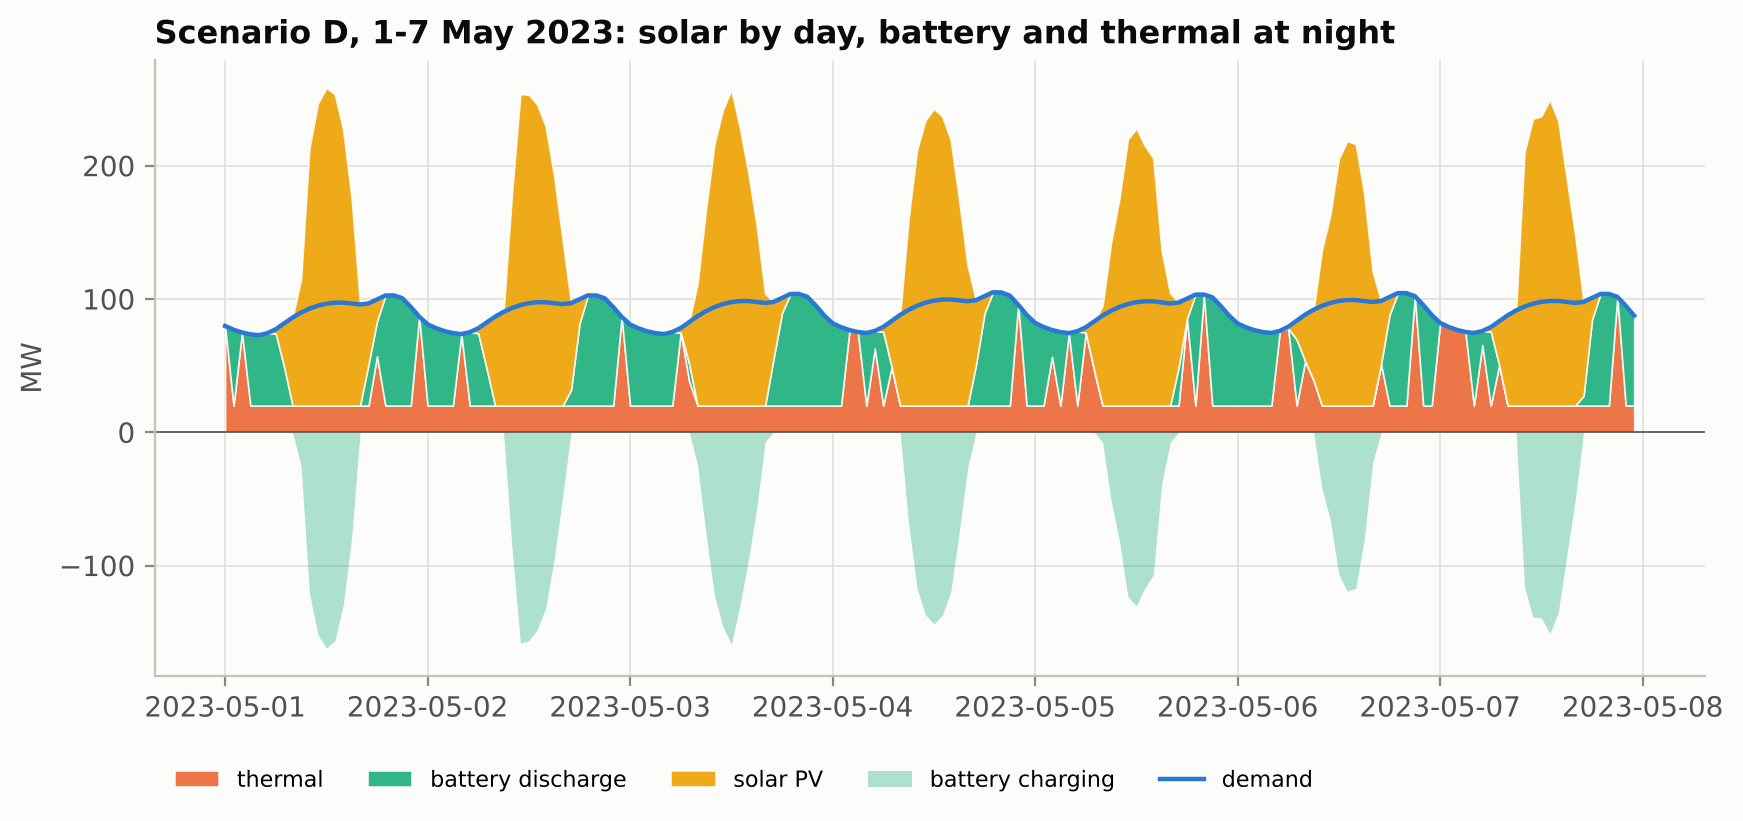
\includegraphics[width=0.95\textwidth]{cs07_week_D.png}
\caption{Scenario D, 1-7 May 2023: solar by day, battery in the evening, thermal must-run at night.}
\end{figure}

\subsection{Step 7: verification}
Solar LCOE if fully used: $86\,943/1\,710 = 51$ \$/MWh $<$ 70 and 180 \$/MWh: PV must be built in every optimised
scenario. \checkmark\ Scenario B: $726$ GWh $\times$ 180 \$/MWh = 130.7 M\$ (same as the output). \checkmark\ The AC load flow
of scenario D stays within 0.968-1.02 p.u.\ and 69\,\% loading. \checkmark

\subsection{Step 8: interpretation}
Without storage the optimum stops at about 154 MW of PV (20\,\% curtailed): midday demand minus the must-run cannot absorb
more. \textbf{Storage, not the grid, unlocks solar}: with a 196 MW / 783 MWh battery, 333 MW of PV supply 72\,\% of the
demand; fuel $-68\,\%$, cost $-22\,\%$ (180 $\to$ 140 \$/MWh). With imports, adding about 145 MW of PV still lowers the cost
from 78 to 68 \$/MWh. The thermal plant stays for the monsoon weeks.
\begin{sayit}
``With real hourly weather for 2023, I optimised investment and operation together. When imports stop, solar plus a
four-hour battery is the least-cost answer and cuts fuel by two thirds; the AC check confirms the plan is feasible.''
\end{sayit}

% ================================================================ real case B
\section{Real case B: off-grid mini-grid in the Agadez region}

\subsection{Step 1: statement and question}
\begin{gbox}{Statement (decision case)}
An isolated town (peak 2 MW) is supplied by diesel generators, with fuel trucked over long distances. What mix of PV and
batteries minimises the cost of electricity, how much diesel does it save, and how robust is the answer to the fuel price
(0.8 to 1.4 \$/litre)?
\end{gbox}

\subsection{Step 2: data and hypotheses}
Real hourly weather 2023 for Agadez (NASA POWER; PV 1\,857 kWh/kWp); demand 12.4 GWh/yr (temperature-driven model);
existing 2.5 MW genset, 0.28 l/kWh, 20 \$/MWh O\&M, 0.74 tCO$_2$/MWh; remote-site PV 1\,000 \$/kW, battery 350 \$/kWh + 200 \$/kW.

\subsection{Step 3: model}
Same capacity-expansion model as case A on a single bus: diesel cost $c_d = 1000\cdot\text{price}\cdot0.28 + 20$ \$/MWh;
cost of electricity $=$ (annualised capital $+$ fuel) / energy.

\subsection{Step 4: method}
Diesel-only reference, optimal hybrid at 1.00 \$/l, then the same optimisation for four fuel prices.

\subsection{Step 5: implementation}
\code{s09_real_case_agadez.py}{Real case B in PyPSA.}

\subsection{Step 6: results}
\progout{s09.txt}{Output of Code 9.}
\begin{figure}[h]\centering
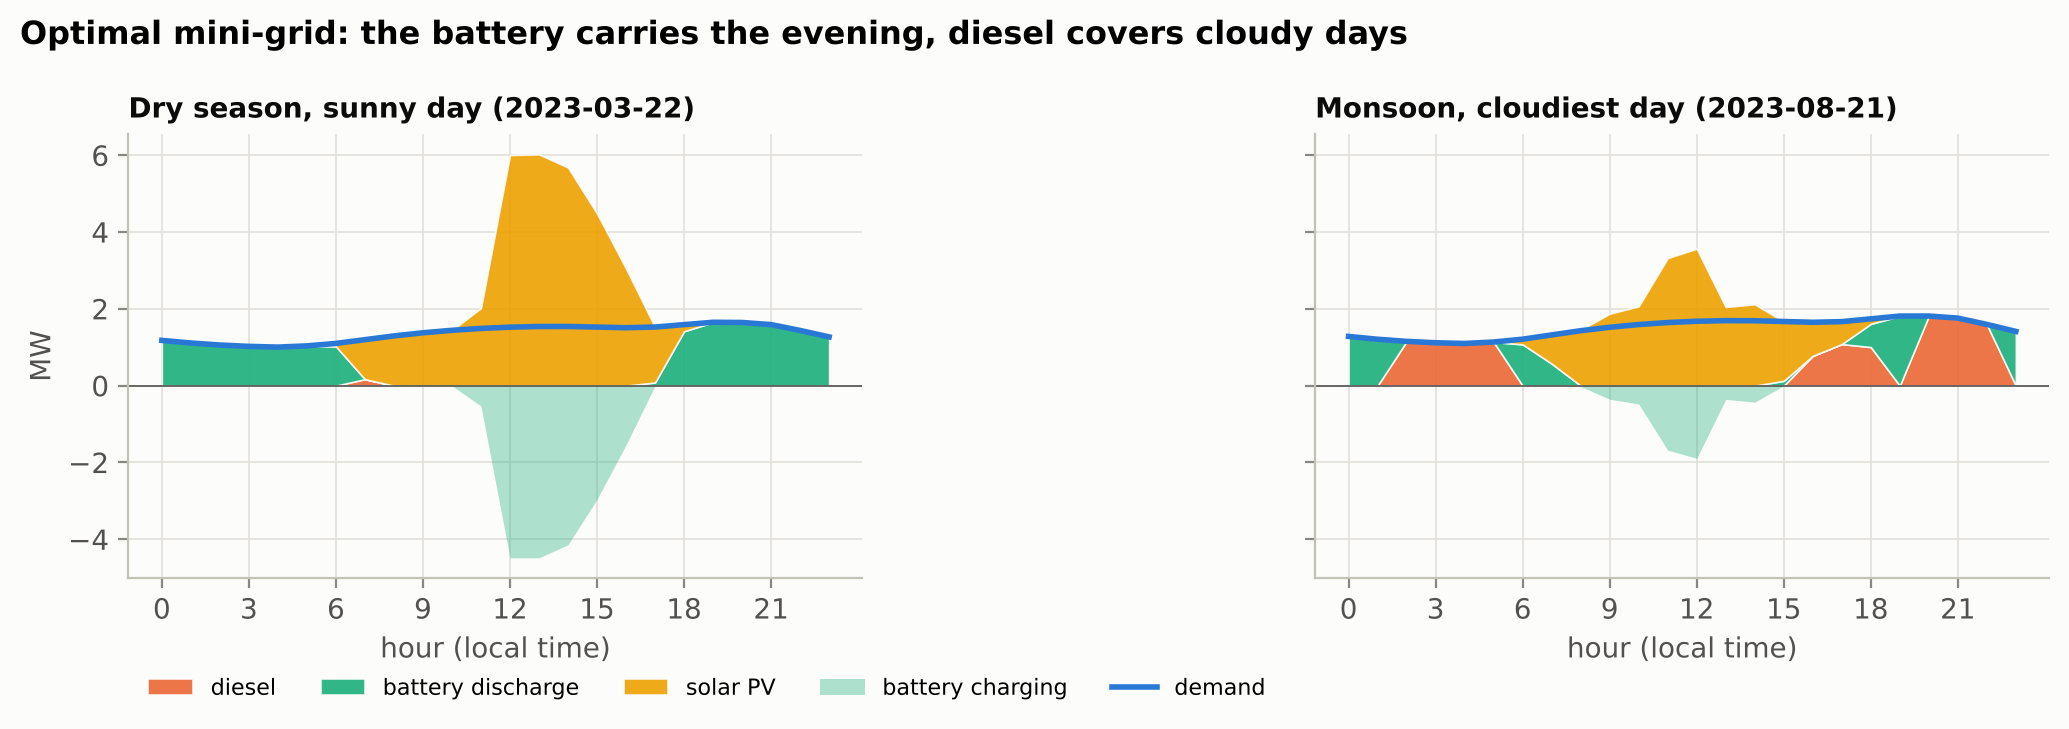
\includegraphics[width=0.95\textwidth]{cs08_typical_days.png}
\caption{Optimal mini-grid: a sunny dry-season day and the cloudiest monsoon day.}
\end{figure}

\subsection{Step 7: verification}
Diesel only: $0.28 \times 1000 + 20 = 300$ \$/MWh $= 0.30$ \$/kWh (no capital cost: existing genset). \checkmark\
Litres: $12\,445$ MWh $\times$ 280 l/MWh = 3.48 million litres. \checkmark

\subsection{Step 8: interpretation}
The hybrid (7.5 MW PV, 18 MWh battery) supplies 94\,\% of the energy, cuts diesel by 94\,\% and the cost from 0.30 to
0.16 \$/kWh; it stays cheaper at every fuel price tested. The genset remains as back-up for cloudy monsoon days.
\begin{sayit}
``For an isolated town, solar plus storage halves the cost of electricity and removes almost all diesel, whatever the fuel
price. The investment replaces a volatile fuel bill by a predictable cost.''
\end{sayit}

% ================================================================ comparison
\section{The cases side by side: what changes}
\begin{table}[h]\centering\small
\caption{Problem, cause, remedy and key number of each case.}
\begin{tabularx}{\textwidth}{@{}l>{\raggedright}p{2.6cm}>{\raggedright}p{3.6cm}>{\raggedright}p{3.3cm}X@{}}
\toprule
Case & Problem & Physical cause & First remedy & Key number \\
\midrule
Ex.\ 5 & state of the grid & non-linear equations & Newton-Raphson & 4 iterations, $|U_3| = 0.951$ \\
TP 1 & power sharing & slack closes the balance & solar reduces thermal & 50.3 $\to$ 20.2 MW \\
TP 2 & undervoltage & long line, reactive load ($X \approx 3R$) & local capacitor bank & 0.919 $\to$ 0.959 p.u. \\
TP 3 & congestion, N-1 & outage redistributes flows & preventive redispatch & 113 $\to$ 99\,\%, 54 \$/h \\
TP 4 & demand growth & reactive reserve exhausted & reactive compensation & limit +77\,\% \\
TP 5 & reverse flow & export raises voltage & set points, inverter Q & 3 $\to$ 129 MW \\
Case A & planning & midday surplus, evening peak & storage & cost $-22\,\%$, fuel $-68\,\%$ \\
Case B & energy access & expensive diesel & PV + battery & 0.30 $\to$ 0.16 \$/kWh \\
\bottomrule
\end{tabularx}
\end{table}

\section{Secrets and pitfalls}
\begin{gbox}{Secret n\textsuperscript{o}1: always check the data before computing}
A load flow that does not converge often has \textbf{no solution}. In Exercise 5 the literal line data cannot carry the
load: swap the values, state the hypothesis, and compare with the other reading.
\end{gbox}
\begin{gbox}{Secret n\textsuperscript{o}2: reactive power moves voltage, active power moves angles}
On transmission lines $X \gg R$: undervoltage is cured by local reactive power (TP 2), overvoltage by absorbing it (TP 5).
\end{gbox}
\begin{gbox}{Secret n\textsuperscript{o}3: enforce generator reactive limits}
PyPSA's \texttt{n.pf()} holds PV voltages whatever reactive power it takes. Without PV $\to$ PQ switching, TP 4 would
claim +145\,\% of loadability instead of +77\,\%.
\end{gbox}
\begin{gbox}{Secret n\textsuperscript{o}4: a linear optimisation must be checked with the AC load flow}
The DC security-constrained OPF of TP 3 fixed the flows but could not see the voltage collapse at bus 9.
\end{gbox}
\begin{gbox}{Secret n\textsuperscript{o}5: PyPSA details that cost hours}
A numeric \texttt{p\_set} \textbf{fixes} a generator in \texttt{n.optimize()} (set it to NaN); the slack needs a numeric
\texttt{p\_set} (0) for \texttt{n.pf()}; lines are in $\Omega$/S, transformers in p.u.\ on their own rating; a solved network
is copied only after \texttt{n.model.solver\_model = None}.
\end{gbox}
\begin{gbox}{Secret n\textsuperscript{o}6: quick plausibility checks}
Active balance (generation = load + losses); $\Delta V \approx (RP + XQ)/V$ on the critical line; losses of a few percent;
voltages 0.9-1.1 p.u.; a result outside these ranges signals a unit or data error.
\end{gbox}

\section{Reflex sheet (to copy at the start of an exam or a study)}
\begin{gbox}{Check-list}
\begin{enumerate}
\item Read the statement; write the question in one sentence; copy the diagram and mark bus types (slack, PV, PQ).
\item List the data with units; convert to PyPSA units ($Z_B = \text{kV}^2/\text{MVA}$); write every hypothesis.
\item Write the model: unknowns, equations, limits (and costs if it is an optimisation).
\item Choose the method: \texttt{n.pf()}, Q-limit loop, \texttt{n.optimize()}, security-constrained OPF, bisection on a limit.
\item Code it; print voltages, flows, loadings, losses.
\item Verify: balances, hand estimate, independent solver, orders of magnitude.
\item Interpret: which bus or line, why (physics), what to do (cheapest effective remedy first).
\item Present in five steps: context, problem, method, results, recommendations.
\end{enumerate}
\end{gbox}

\end{document}
